%%%%%%%%%%%%%%%%%%%%%%%%%%%%%%%%%%%%%%%%%
% The Legrand Orange Book
% LaTeX Template
% Version 2.0 (9/2/15)
%
% This template has been downloaded from:
% http://www.LaTeXTemplates.com
%
% Mathias Legrand (legrand.mathias@gmail.com) with modifications by:
% Vel (vel@latextemplates.com)
%
% License:
% CC BY-NC-SA 3.0 (http://creativecommons.org/licenses/by-nc-sa/3.0/)
%
% Compiling this template:
% This template uses biber for its bibliography and makeindex for its index.
% When you first open the template, compile it from the command line with the 
% commands below to make sure your LaTeX distribution is configured correctly:
%
% 1) pdflatex main
% 2) makeindex main.idx -s StyleInd.ist
% 3) biber main
% 4) pdflatex main x 2
%
% After this, when you wish to update the bibliography/index use the appropriate
% command above and make sure to compile with pdflatex several times 
% afterwards to propagate your changes to the document.
%
% This template also uses a number of packages which may need to be
% updated to the newest versions for the template to compile. It is strongly
% recommended you update your LaTeX distribution if you have any
% compilation errors.
%
% Important note:
% Chapter heading images should have a 2:1 width:height ratio,
% e.g. 920px width and 460px height.
%
%%%%%%%%%%%%%%%%%%%%%%%%%%%%%%%%%%%%%%%%%

%----------------------------------------------------------------------------------------
%	PACKAGES AND OTHER DOCUMENT CONFIGURATIONS
%----------------------------------------------------------------------------------------

\documentclass[12pt,fleqn, twoside, letter]{book} 
% Default font size and left-justified equations

%----------------------------------------------------------------------------------------
%%%%%%%%%%%%%%%%%%%%%%%%%%%%%%%%%%%%%%%%%
% The Legrand Orange Book
% Structural Definitions File
% Version 2.0 (9/2/15)
%
% Original author:
% Mathias Legrand (legrand.mathias@gmail.com) with modifications by:
% Vel (vel@latextemplates.com)
% 
% This file has been downloaded from:
% http://www.LaTeXTemplates.com
%
% License:
% CC BY-NC-SA 3.0 (http://creativecommons.org/licenses/by-nc-sa/3.0/)
%
%%%%%%%%%%%%%%%%%%%%%%%%%%%%%%%%%%%%%%%%%

%----------------------------------------------------------------------------------------
%	VARIOUS REQUIRED PACKAGES AND CONFIGURATIONS
%----------------------------------------------------------------------------------------

\usepackage[top=3cm,bottom=3cm,left=3cm,right=3cm,headsep=10pt,a4paper]{geometry} % Page margins

\usepackage{graphicx} % Required for including pictures
\graphicspath{{Pictures/}} % Specifies the directory where pictures are stored

\usepackage{lipsum} % Inserts dummy text

\usepackage{tikz} % Required for drawing custom shapes

\usepackage[spanish]{babel} % English language/hyphenation

\usepackage{enumitem} % Customize lists
\setlist{nolistsep} % Reduce spacing between bullet points and numbered lists

\usepackage{booktabs} % Required for nicer horizontal rules in tables

\usepackage{xcolor} % Required for specifying colors by name
%\definecolor{ocre}{RGB}{243,102,25} % Define the orange color used for highlighting throughout the book
\definecolor{ocre}{RGB}{80,97,123} % Define the orange color used for highlighting throughout the book

%----------------------------------------------------------------------------------------
%	FONTS
%----------------------------------------------------------------------------------------

\usepackage{avant} % Use the Avantgarde font for headings
%\usepackage{times} % Use the Times font for headings
\usepackage{mathptmx} % Use the Adobe Times Roman as the default text font together with math symbols from the Sym­bol, Chancery and Com­puter Modern fonts

\usepackage{microtype} % Slightly tweak font spacing for aesthetics
\usepackage[utf8]{inputenc} % Required for including letters with accents
\usepackage[T1]{fontenc} % Use 8-bit encoding that has 256 glyphs

%----------------------------------------------------------------------------------------
%	BIBLIOGRAPHY AND INDEX
%----------------------------------------------------------------------------------------

\usepackage[babel]{csquotes}
%%%%\usepackage[backend=biber,style=apa]{biblatex}
\usepackage[style=apa]{biblatex}
\DeclareLanguageMapping{spanish}{spanish-apa}

\addbibresource{bibliography.bib} % BibTeX bibliography file
\defbibheading{bibempty}{}

%%%%

\usepackage{calc} % For simpler calculation - used for spacing the index letter headings correctly
\usepackage{makeidx} % Required to make an index
\makeindex % Tells LaTeX to create the files required for indexing

%----------------------------------------------------------------------------------------
%	MAIN TABLE OF CONTENTS
%----------------------------------------------------------------------------------------

\usepackage{titletoc} % Required for manipulating the table of contents

\contentsmargin{0cm} % Removes the default margin

% Part text styling
\titlecontents{part}[0cm]
{\addvspace{20pt}\centering\large\bfseries}
{}
{}
{}

% Chapter text styling
\titlecontents{chapter}[1.25cm] % Indentation
{\addvspace{12pt}\large\sffamily\bfseries} % Spacing and font options for chapters
{\color{ocre!60}\contentslabel[\Large\thecontentslabel]{1.25cm}\color{ocre}} % Chapter number
{\color{ocre}}  
{\color{ocre!60}\normalsize\;\titlerule*[.5pc]{.}\;\thecontentspage} % Page number

% Section text styling
\titlecontents{section}[1.25cm] % Indentation
{\addvspace{3pt}\sffamily\bfseries} % Spacing and font options for sections
{\contentslabel[\thecontentslabel]{1.25cm}} % Section number
{}
{\hfill\color{black}\thecontentspage} % Page number
[]

% Subsection text styling
\titlecontents{subsection}[1.25cm] % Indentation
{\addvspace{1pt}\sffamily\small} % Spacing and font options for subsections
{\contentslabel[\thecontentslabel]{1.25cm}} % Subsection number
{}
{\ \titlerule*[.5pc]{.}\;\thecontentspage} % Page number
[]

% List of figures
\titlecontents{figure}[0em]
{\addvspace{-5pt}\sffamily}
{\thecontentslabel\hspace*{1em}}
{}
{\ \titlerule*[.5pc]{.}\;\thecontentspage}
[]

% List of tables
\titlecontents{table}[0em]
{\addvspace{-5pt}\sffamily}
{\thecontentslabel\hspace*{1em}}
{}
{\ \titlerule*[.5pc]{.}\;\thecontentspage}
[]

%----------------------------------------------------------------------------------------
%	MINI TABLE OF CONTENTS IN PART HEADS
%----------------------------------------------------------------------------------------

% Chapter text styling
\titlecontents{lchapter}[0em] % Indenting
{\addvspace{15pt}\large\sffamily\bfseries} % Spacing and font options for chapters
{\color{ocre}\contentslabel[\Large\thecontentslabel]{1.25cm}\color{ocre}} % Chapter number
{}  
{\color{ocre}\normalsize\sffamily\bfseries\;\titlerule*[.5pc]{.}\;\thecontentspage} % Page number

% Section text styling
\titlecontents{lsection}[0em] % Indenting
{\sffamily\small} % Spacing and font options for sections
{\contentslabel[\thecontentslabel]{1.25cm}} % Section number
{}
{}

% Subsection text styling
\titlecontents{lsubsection}[.5em] % Indentation
{\normalfont\footnotesize\sffamily} % Font settings
{}
{}
{}

%----------------------------------------------------------------------------------------
%	PAGE HEADERS
%----------------------------------------------------------------------------------------

\usepackage{fancyhdr} % Required for header and footer configuration

\pagestyle{fancy}
\renewcommand{\chaptermark}[1]{\markboth{\sffamily\normalsize\bfseries\chaptername\ \thechapter.\ #1}{}} % Chapter text font settings
\renewcommand{\sectionmark}[1]{\markright{\sffamily\normalsize\thesection\hspace{5pt}#1}{}} % Section text font settings
\fancyhf{} \fancyhead[LE,RO]{\sffamily\normalsize\thepage} % Font setting for the page number in the header
\fancyhead[LO]{\rightmark} % Print the nearest section name on the left side of odd pages
\fancyhead[RE]{\leftmark} % Print the current chapter name on the right side of even pages
\renewcommand{\headrulewidth}{0.5pt} % Width of the rule under the header
\addtolength{\headheight}{2.5pt} % Increase the spacing around the header slightly
\renewcommand{\footrulewidth}{0pt} % Removes the rule in the footer
\fancypagestyle{plain}{\fancyhead{}\renewcommand{\headrulewidth}{0pt}} % Style for when a plain pagestyle is specified

% Removes the header from odd empty pages at the end of chapters
\makeatletter
\renewcommand{\cleardoublepage}{
\clearpage\ifodd\c@page\else
\hbox{}
\vspace*{\fill}
\thispagestyle{empty}
\newpage
\fi}

%----------------------------------------------------------------------------------------
%	THEOREM STYLES
%----------------------------------------------------------------------------------------

\usepackage{amsmath,amsfonts,amssymb,amsthm} % For math equations, theorems, symbols, etc

\newcommand{\intoo}[2]{\mathopen{]}#1\,;#2\mathclose{[}}
\newcommand{\ud}{\mathop{\mathrm{{}d}}\mathopen{}}
\newcommand{\intff}[2]{\mathopen{[}#1\,;#2\mathclose{]}}
\newtheorem{notation}{Notation}[chapter]

% Boxed/framed environments
\newtheoremstyle{ocrenumbox}% % Theorem style name
{0pt}% Space above
{0pt}% Space below
{\normalfont}% % Body font
{}% Indent amount
{\small\bf\sffamily\color{ocre}}% % Theorem head font
{\;}% Punctuation after theorem head
{0.25em}% Space after theorem head
{\small\sffamily\color{ocre}\thmname{#1}\nobreakspace\thmnumber{\@ifnotempty{#1}{}\@upn{#2}}% Theorem text (e.g. Theorem 2.1)
\thmnote{\nobreakspace\the\thm@notefont\sffamily\bfseries\color{black}---\nobreakspace#3.}} % Optional theorem note
\renewcommand{\qedsymbol}{$\blacksquare$}% Optional qed square

\newtheoremstyle{blacknumex}% Theorem style name
{5pt}% Space above
{5pt}% Space below
{\normalfont}% Body font
{} % Indent amount
{\small\bf\sffamily}% Theorem head font
{\;}% Punctuation after theorem head
{0.25em}% Space after theorem head
{\small\sffamily{\tiny\ensuremath{\blacksquare}}\nobreakspace\thmname{#1}\nobreakspace\thmnumber{\@ifnotempty{#1}{}\@upn{#2}}% Theorem text (e.g. Theorem 2.1)
\thmnote{\nobreakspace\the\thm@notefont\sffamily\bfseries---\nobreakspace#3.}}% Optional theorem note

\newtheoremstyle{blacknumbox} % Theorem style name
{0pt}% Space above
{0pt}% Space below
{\normalfont}% Body font
{}% Indent amount
{\small\bf\sffamily}% Theorem head font
{\;}% Punctuation after theorem head
{0.25em}% Space after theorem head
{\small\sffamily\thmname{#1}\nobreakspace\thmnumber{\@ifnotempty{#1}{}\@upn{#2}}% Theorem text (e.g. Theorem 2.1)
\thmnote{\nobreakspace\the\thm@notefont\sffamily\bfseries---\nobreakspace#3.}}% Optional theorem note

% Non-boxed/non-framed environments
\newtheoremstyle{ocrenum}% % Theorem style name
{5pt}% Space above
{5pt}% Space below
{\normalfont}% % Body font
{}% Indent amount
{\small\bf\sffamily\color{ocre}}% % Theorem head font
{\;}% Punctuation after theorem head
{0.25em}% Space after theorem head
{\small\sffamily\color{ocre}\thmname{#1}\nobreakspace\thmnumber{\@ifnotempty{#1}{}\@upn{#2}}% Theorem text (e.g. Theorem 2.1)
\thmnote{\nobreakspace\the\thm@notefont\sffamily\bfseries\color{black}---\nobreakspace#3.}} % Optional theorem note
\renewcommand{\qedsymbol}{$\blacksquare$}% Optional qed square
\makeatother

% Defines the theorem text style for each type of theorem to one of the three styles above
\newcounter{dummy} 
\numberwithin{dummy}{section}
\theoremstyle{ocrenumbox}
\newtheorem{theoremeT}[dummy]{Theorem}
\newtheorem{problem}{Problem}[chapter]
\newtheorem{exerciseT}{Exercise}[chapter]
\theoremstyle{blacknumex}
\newtheorem{exampleT}{Example}[chapter]
\theoremstyle{blacknumbox}
\newtheorem{vocabulary}{Vocabulary}[chapter]
\newtheorem{definitionT}{Definition}[section]
\newtheorem{corollaryT}[dummy]{Corollary}
\theoremstyle{ocrenum}
\newtheorem{proposition}[dummy]{Proposition}

%----------------------------------------------------------------------------------------
%	DEFINITION OF COLORED BOXES
%----------------------------------------------------------------------------------------

\RequirePackage[framemethod=default]{mdframed} % Required for creating the theorem, definition, exercise and corollary boxes

% Theorem box
\newmdenv[skipabove=7pt,
skipbelow=7pt,
backgroundcolor=black!5,
linecolor=ocre,
innerleftmargin=5pt,
innerrightmargin=5pt,
innertopmargin=5pt,
leftmargin=0cm,
rightmargin=0cm,
innerbottommargin=5pt]{tBox}

% Exercise box	  
\newmdenv[skipabove=7pt,
skipbelow=7pt,
rightline=false,
leftline=true,
topline=false,
bottomline=false,
backgroundcolor=ocre!10,
linecolor=ocre,
innerleftmargin=5pt,
innerrightmargin=5pt,
innertopmargin=5pt,
innerbottommargin=5pt,
leftmargin=0cm,
rightmargin=0cm,
linewidth=4pt]{eBox}	

% Definition box
\newmdenv[skipabove=7pt,
skipbelow=7pt,
rightline=false,
leftline=true,
topline=false,
bottomline=false,
linecolor=ocre,
innerleftmargin=5pt,
innerrightmargin=5pt,
innertopmargin=0pt,
leftmargin=0cm,
rightmargin=0cm,
linewidth=4pt,
innerbottommargin=0pt]{dBox}	

% Corollary box
\newmdenv[skipabove=7pt,
skipbelow=7pt,
rightline=false,
leftline=true,
topline=false,
bottomline=false,
linecolor=gray,
backgroundcolor=black!5,
innerleftmargin=5pt,
innerrightmargin=5pt,
innertopmargin=5pt,
leftmargin=0cm,
rightmargin=0cm,
linewidth=4pt,
innerbottommargin=5pt]{cBox}

% Creates an environment for each type of theorem and assigns it a theorem text style from the "Theorem Styles" section above and a colored box from above
\newenvironment{theorem}{\begin{tBox}\begin{theoremeT}}{\end{theoremeT}\end{tBox}}
\newenvironment{exercise}{\begin{eBox}\begin{exerciseT}}{\hfill{\color{ocre}\tiny\ensuremath{\blacksquare}}\end{exerciseT}\end{eBox}}				  
\newenvironment{definition}{\begin{dBox}\begin{definitionT}}{\end{definitionT}\end{dBox}}	
\newenvironment{example}{\begin{exampleT}}{\hfill{\tiny\ensuremath{\blacksquare}}\end{exampleT}}		
\newenvironment{corollary}{\begin{cBox}\begin{corollaryT}}{\end{corollaryT}\end{cBox}}	

%----------------------------------------------------------------------------------------
%	REMARK ENVIRONMENT
%----------------------------------------------------------------------------------------

\newenvironment{remark}{\par\vspace{10pt}\small % Vertical white space above the remark and smaller font size
\begin{list}{}{
\leftmargin=35pt % Indentation on the left
\rightmargin=25pt}\item\ignorespaces % Indentation on the right
\makebox[-2.5pt]{\begin{tikzpicture}[overlay]
\node[draw=ocre!60,line width=1pt,circle,fill=ocre!25,font=\sffamily\bfseries,inner sep=2pt,outer sep=0pt] at (-15pt,0pt){\textcolor{ocre}{R}};\end{tikzpicture}} % Orange R in a circle
\advance\baselineskip -1pt}{\end{list}\vskip5pt} % Tighter line spacing and white space after remark

%----------------------------------------------------------------------------------------
%	SECTION NUMBERING IN THE MARGIN
%----------------------------------------------------------------------------------------

\makeatletter
\renewcommand{\@seccntformat}[1]{\llap{\textcolor{ocre}{\csname the#1\endcsname}\hspace{1em}}}                    
\renewcommand{\section}{\@startsection{section}{1}{\z@}
{-4ex \@plus -1ex \@minus -.4ex}
{1ex \@plus.2ex }
{\normalfont\large\sffamily\bfseries}}
\renewcommand{\subsection}{\@startsection {subsection}{2}{\z@}
{-3ex \@plus -0.1ex \@minus -.4ex}
{0.5ex \@plus.2ex }
{\normalfont\sffamily\bfseries}}
\renewcommand{\subsubsection}{\@startsection {subsubsection}{3}{\z@}
{-2ex \@plus -0.1ex \@minus -.2ex}
{.2ex \@plus.2ex }
{\normalfont\small\sffamily\bfseries}}                        
\renewcommand\paragraph{\@startsection{paragraph}{4}{\z@}
{-2ex \@plus-.2ex \@minus .2ex}
{.1ex}
{\normalfont\small\sffamily\bfseries}}

%----------------------------------------------------------------------------------------
%	PART HEADINGS
%----------------------------------------------------------------------------------------

% numbered part in the table of contents
\newcommand{\@mypartnumtocformat}[2]{%
\setlength\fboxsep{0pt}%
\noindent\colorbox{ocre!20}{\strut\parbox[c][.7cm]{\ecart}{\color{ocre!70}\Large\sffamily\bfseries\centering#1}}\hskip\esp\colorbox{ocre!40}{\strut\parbox[c][.7cm]{\linewidth-\ecart-\esp}{\Large\sffamily\centering#2}}}%
%%%%%%%%%%%%%%%%%%%%%%%%%%%%%%%%%%
% unnumbered part in the table of contents
\newcommand{\@myparttocformat}[1]{%
\setlength\fboxsep{0pt}%
\noindent\colorbox{ocre!40}{\strut\parbox[c][.7cm]{\linewidth}{\Large\sffamily\centering#1}}}%
%%%%%%%%%%%%%%%%%%%%%%%%%%%%%%%%%%
\newlength\esp
\setlength\esp{4pt}
\newlength\ecart
\setlength\ecart{1.2cm-\esp}
\newcommand{\thepartimage}{}%
\newcommand{\partimage}[1]{\renewcommand{\thepartimage}{#1}}%
\def\@part[#1]#2{%
\ifnum \c@secnumdepth >-2\relax%
\refstepcounter{part}%
\addcontentsline{toc}{part}{\texorpdfstring{\protect\@mypartnumtocformat{\thepart}{#1}}{\partname~\thepart\ ---\ #1}}
\else%
\addcontentsline{toc}{part}{\texorpdfstring{\protect\@myparttocformat{#1}}{#1}}%
\fi%
\startcontents%
\markboth{}{}%
{\thispagestyle{empty}%
\begin{tikzpicture}[remember picture,overlay]%
\node at (current page.north west){\begin{tikzpicture}[remember picture,overlay]%	
\fill[ocre!20](0cm,0cm) rectangle (\paperwidth,-\paperheight);
\node[anchor=north] at (4cm,-3.25cm){\color{ocre!40}\fontsize{220}{100}\sffamily\bfseries\@Roman\c@part}; 
\node[anchor=south east] at (\paperwidth-1cm,-\paperheight+1cm){\parbox[t][][t]{8.5cm}{
\printcontents{l}{0}{\setcounter{tocdepth}{1}}%
}};
\node[anchor=north east] at (\paperwidth-1.5cm,-3.25cm){\parbox[t][][t]{15cm}{\strut\raggedleft\color{white}\fontsize{30}{30}\sffamily\bfseries#2}};
\end{tikzpicture}};
\end{tikzpicture}}%
\@endpart}
\def\@spart#1{%
\startcontents%
\phantomsection
{\thispagestyle{empty}%
\begin{tikzpicture}[remember picture,overlay]%
\node at (current page.north west){\begin{tikzpicture}[remember picture,overlay]%	
\fill[ocre!20](0cm,0cm) rectangle (\paperwidth,-\paperheight);
\node[anchor=north east] at (\paperwidth-1.5cm,-3.25cm){\parbox[t][][t]{15cm}{\strut\raggedleft\color{white}\fontsize{30}{30}\sffamily\bfseries#1}};
\end{tikzpicture}};
\end{tikzpicture}}
\addcontentsline{toc}{part}{\texorpdfstring{%
\setlength\fboxsep{0pt}%
\noindent\protect\colorbox{ocre!40}{\strut\protect\parbox[c][.7cm]{\linewidth}{\Large\sffamily\protect\centering #1\quad\mbox{}}}}{#1}}%
\@endpart}
\def\@endpart{\vfil\newpage
\if@twoside
\if@openright
\null
\thispagestyle{empty}%
\newpage
\fi
\fi
\if@tempswa
\twocolumn
\fi}

%----------------------------------------------------------------------------------------
%	CHAPTER HEADINGS
%----------------------------------------------------------------------------------------

\newcommand{\thechapterimage}{}%
\newcommand{\chapterimage}[1]{\renewcommand{\thechapterimage}{#1}}%
\def\@makechapterhead#1{%
{\parindent \z@ \raggedright \normalfont
\ifnum \c@secnumdepth >\m@ne
\if@mainmatter
\begin{tikzpicture}[remember picture,overlay]
\node at (current page.north west)
{\begin{tikzpicture}[remember picture,overlay]
\node[anchor=north west,inner sep=0pt] at (0,0) {\includegraphics[width=\paperwidth]{\thechapterimage}};
\draw[anchor=west] (\Gm@lmargin,-9cm) node [line width=2pt,rounded corners=15pt,draw=ocre,fill=white,fill opacity=0.5,inner sep=15pt]{\strut\makebox[22cm]{}};
\draw[anchor=west] (\Gm@lmargin+.3cm,-9cm) node {\huge\sffamily\bfseries\color{black}\thechapter. #1\strut};
\end{tikzpicture}};
\end{tikzpicture}
\else
\begin{tikzpicture}[remember picture,overlay]
\node at (current page.north west)
{\begin{tikzpicture}[remember picture,overlay]
\node[anchor=north west,inner sep=0pt] at (0,0) {\includegraphics[width=\paperwidth]{\thechapterimage}};
\draw[anchor=west] (\Gm@lmargin,-9cm) node [line width=2pt,rounded corners=15pt,draw=ocre,fill=white,fill opacity=0.5,inner sep=15pt]{\strut\makebox[22cm]{}};
\draw[anchor=west] (\Gm@lmargin+.3cm,-9cm) node {\huge\sffamily\bfseries\color{black}#1\strut};
\end{tikzpicture}};
\end{tikzpicture}
\fi\fi\par\vspace*{270\p@}}}

%-------------------------------------------

\def\@makeschapterhead#1{%
\begin{tikzpicture}[remember picture,overlay]
\node at (current page.north west)
{\begin{tikzpicture}[remember picture,overlay]
\node[anchor=north west,inner sep=0pt] at (0,0) {\includegraphics[width=\paperwidth]{\thechapterimage}};
\draw[anchor=west] (\Gm@lmargin,-9cm) node [line width=2pt,rounded corners=15pt,draw=ocre,fill=white,fill opacity=0.5,inner sep=15pt]{\strut\makebox[22cm]{}};
\draw[anchor=west] (\Gm@lmargin+.3cm,-9cm) node {\huge\sffamily\bfseries\color{black}#1\strut};
\end{tikzpicture}};
\end{tikzpicture}
\par\vspace*{270\p@}}
\makeatother

%----------------------------------------------------------------------------------------
%	HYPERLINKS IN THE DOCUMENTS
%----------------------------------------------------------------------------------------

\usepackage{hyperref}
\hypersetup{
	hidelinks,
	colorlinks=true,
	breaklinks=true,
	urlcolor= cyan,
	linkcolor=cyan,
	citecolor = cyan,
	bookmarksopen=false,
	pdftitle={Title},
	pdfauthor={Author}
}

%\hypersetup{hidelinks,backref=true,pagebackref=true,hyperindex=true,colorlinks=blue,breaklinks=true,urlcolor= ocre,bookmarks=true,bookmarksopen=false,pdftitle={Title},pdfauthor={Author}}

\usepackage{bookmark}
\bookmarksetup{
open,
numbered,
addtohook={%
\ifnum\bookmarkget{level}=0 % chapter
\bookmarksetup{bold}%
\fi
\ifnum\bookmarkget{level}=-1 % part
\bookmarksetup{color=ocre,bold}%
\fi
}
}

%% Para simulación de consola
\usepackage[most]{tcolorbox}

\newtcblisting{commandshell}{
colback=black,
colupper=white,
colframe=white!55!black,
listing only,
listing options={language=sh},
every listing line={\textcolor{white}{\small\ttfamily\bfseries \$ }}}

\newtcblisting{commandshellroot}{
colback=black,
colupper=white,
colframe=white!75!black,
listing only,
listing options={language=sh},
every listing line={\textcolor{white}{\small\ttfamily\bfseries \# }}} % Insert the commands.tex file which contains the majority of the structure behind the template

\usepackage[hang, small,labelfont=bf,up,textfont=it,up]{caption} % Custom captions under/above floats in tables or figures
\usepackage{booktabs} % Horizontal rules in tables
\usepackage{float} % Required for tables and figures in the multi-column environment - they

\usepackage{graphicx} % paquete que permite introducir imágenes

\usepackage{booktabs} % Horizontal rules in tables
\usepackage{float} % Required for tables and figures in the multi-column environment - they

\usepackage{ftnxtra} % Permite color los pie de página en el Caption de las figuras.


\numberwithin{equation}{section} % Number equations within sections (i.e. 1.1, 1.2, 2.1, 2.2 instead of 1, 2, 3, 4)
\numberwithin{figure}{section} % Number figures within sections (i.e. 1.1, 1.2, 2.1, 2.2 instead of 1, 2, 3, 4)
\numberwithin{table}{section} % Number tables within sections (i.e. 1.1, 1.2, 2.1, 2.2 instead of 1, 2, 3, 4)


\setlength\parindent{0pt} % Removes all indentation from paragraphs - comment this line for an assignment with lots of text


\begin{document}
	
	%----------------------------------------------------------------------------------------
	%	TITLE PAGE
	%----------------------------------------------------------------------------------------
	
	\begingroup
	\thispagestyle{empty}
	\begin{tikzpicture}[remember picture,overlay]
	\coordinate [below=12cm] (midpoint) at (current page.north);
	\node at (current page.north west)
	{\begin{tikzpicture}[remember picture,overlay]
		\node[anchor=north west,inner sep=0pt] at (0,0) {
\includegraphics[width=\paperwidth]{backgroundBook}}; 
		% Background image
		%\draw[anchor=north] (midpoint) node [fill=ocre!30!white,fill opacity=0.6,text opacity=1,inner sep=1cm]{\Huge\centering\bfseries\sffamily\parbox[c][][t]{\paperwidth}{\centering Tecnologías de Virtualización\\[15pt] % Book title
		
		\draw[anchor=north] (midpoint) node [text opacity=1,inner sep=1cm]{\Huge\centering\bfseries\sffamily\parbox[c][][t]{\paperwidth}{\centering Recursos educativos para la enseñanza de las Tecnologías de Virtualización\\[15pt] % Book title
				
				{\Large Universidad del Quindío}\\[20pt] % Subtitle
				
				{\huge Luis Eduardo Sepúlveda Rodríguez}}}; % Author name
		\end{tikzpicture}};
\end{tikzpicture}
\vfill
\endgroup


%----------------------------------------------------------------------------------------
%	COPYRIGHT PAGE
%----------------------------------------------------------------------------------------

\newpage
~\vfill
\thispagestyle{empty}

\noindent \textbf{\textsc{Recursos educativos para la enseñanza de las \\Tecnologías de Virtualización}}\\ % Publisher

\noindent Copyright \copyright\ 2019\\
Luis Eduardo Sepúlveda Rodríguez\\

\noindent \textsc{Universidad del Quindío \\ Facultad de Ingeniería \\Ingeniería de Sistemas y Computación}\\

\noindent \textsc{www.uniquindio.edu.co}\\

\noindent Trabajo presentado para el ascenso a la categoría Asociado del escalafón docente en la Universidad del Quindío.\\ 



\includegraphics[]{Pictures/cc-88x31.png}\\
\noindent Este obra está bajo una licencia de Creative Commons Reconocimiento-NoComercial 4.0 Internacional.\\

\noindent \textit{Enero 2019} 

\newpage
%~\vfill
%\thispagestyle{fancy}

%\chapter*{Presentación}
%\markboth{Presentacion}{Presentacion}

{\huge \textbf{Presentación}}\\

Este documento corresponde al trabajo presentado como requisito para el ascenso en el escalafón docente de la categoría de \textit{Profesor Asociado} en la Universidad del Quindío. Tal como se establece en el Artículo 4o del Acuerdo del Consejo Superior número 010 del 4 de marzo de 1996 \parencite{UQ1996}.\\

La propuesta presentada, se centra en las tecnologías de virtualización y busca  realizar una revisión bibliográfica que permita la descripción de fundamentos, contexto histórico y ámbitos de aplicación de estas tecnologías. Todo esto para la construcción de un conjunto de recursos educativos orientados a la enseñanza de las tecnologías de virtualización, buscando un aporte significativo a la docencia, especialmente en los espacios académicos del área de infraestructura de Tecnología Informática (TI) del programa de Ingeniería de Sistemas y Computación en la Facultad de Ingeniería en la Universidad del Quindío.\\

La virtualización según lo señala \textcite{Goldworm2007} y \textcite{Kusnetzky2011} es una mezcla de tecnologías que permiten realizar una abstracción del hardware presentándolo como una vista lógica del mismo, lo que permite que múltiples “máquinas virtuales” se ejecuten en una misma máquina física ( o real). Esta situación trae consigo un esquema de trabajo con mayor flexibilidad, que a su vez facilita la adaptación de la infraestructura de TI hacia las necesidades de las organizaciones. El concepto de tecnologías de virtualización utilizado en esta propuesta, está suscrito en la taxonomía descrita por \textcite{Pessolani2012}, que a su vez cumple los requisitos asociados a la virtualización concebidos por \textcite{Popek1974}. Partiendo de dicha taxonomía, esta propuesta se basa en los siguientes aspectos: a) Virtualización de hardware, b) Para-virtualización, y c) Virtualización basada en sistema operativo. La razón de los aspectos a considerar tiene relación con los contenidos programáticos de los espacios académicos del área de infraestructura de TI del Programa Ingeniería de Sistemas y Computación.\\

Cabe resaltar la actualidad y el impacto de la temática a tratar en la presente propuesta, toda vez que gran parte de las organizaciones hoy en día utilizan la tecnología computacional como un elemento fundamental para potenciar el cumplimiento de sus objetivos \parencite{Pessolani2012}, por lo que se hace necesario contar con el conocimiento preciso acerca de la especificación dinámica de recursos computacionales utilizando tecnologías de virtualización \parencite{Hui2014}. También es importante reconocer y saber gestionar las tecnologías de virtualización que hacen posible soportar el despliegue de recursos tecnológicos en soluciones empresariales de bajo, mediano y alto impacto \parencite{Chiueh2005}. \\

El trabajo presentado consta de dos partes, la Parte \ref{Parte1}, corresponde a la descripción general de la propuesta presentada ante el Consejo de la Facultad de Ingeniería en la Universidad del Quindío. A su vez, esta parte comprende las siguientes secciones: \ref{justificacion}) Justificación, \ref{Objetivos}) Objetivos y \ref{tematicaADesarrollar}) Temática a desarrollar. Es importante dar claridad al lector que los objetivos y alcance de la propuesta fueron aprobados por el Consejo de la Facultad de Ingeniería, mediante el acta No. 16 del 16 de agosto de 2018. La Parte \ref{Parte2}, corresponde al trabajo de ascenso desarrollado, el cual incluye secciones como  \ref{Introduccion}) Introducción, el  \ref{marcoConceptual}) marco conceptual que a su vez comprende \ref{fundamentos}) fundamentos, XXX) contexto histórico y XXX) ámbitos de aplicación, identificación de herramientas de virtualización y recursos educativos acerca de las tecnologías de virtualización entre otras.\\
%----------------------------------------------------------------------------------------
%	TABLE OF CONTENTS
%----------------------------------------------------------------------------------------

\chapterimage{backgroundIndice} % Table of contents heading image
\pagestyle{empty} % No headers
\tableofcontents % Print the table of contents itself
\cleardoublepage % Forces the first chapter to start on an odd page so it's on the right
\pagestyle{fancy} % Print headers again

%----------------------------------------------------------------------------------------
%	PART
%----------------------------------------------------------------------------------------
\part{Propuesta}\label{Parte1}

\chapterimage{chapterImage} % Chapter heading image
\chapter{Justificación}\label{justificacion}
En concordancia con el Plan de Desarrollo Profesoral \parencite{UQPlanDesarrolloPro2016},  y el Proyecto Educativo de la Facultad de Ingeniería \parencite{UQProyectoEducativoFacultad}, el programa de Ingeniería de Sistemas y Computación de la Universidad del Quindío, en el primer semestre de 2017 definió una reforma curricular \parencite{UQACA075}, en la cual se destaca la creación del área de profundización denominada Infraestructura de Tecnología Informática (TI), la cual comprende entre otros espacios académicos los siguientes: \textit{Infraestructura Computacional}, \textit{Administración de Infraestructura}, \textit{Gestión de Servicios de TI } y \textit{Computación en la Nube}; estos espacios académicos tienen relación con las tecnologías de virtualización e incluso algunos lo han declarado explícitamente en su \textit{syllabus}. Por esta razón el presente trabajo genera un apoyo directo al ejercicio docente de estos espacios académicos, al igual que se esperan beneficios indirectos a la demás comunidad académica de la Facultad de Ingeniería en la Universidad del Quindío y demás instituciones de educación con necesidades similares.\\

El conocimiento y utilización de las tecnologías de virtualización en instituciones de educación superior y particularmente en la Universidad del Quindío, puede considerarse como una acción estratégica en el sentido de que se pueden aprovechar al máximo los recursos computacionales existentes \parencite{Klement2017}, permitiendo la generación de escenarios para la construcción de laboratorios virtuales en diversos espacios académicos, estos laboratorios generan un alto valor académico sin incurrir en nuevas inversiones en TI.
\\

Para cualquier comunidad académica es de gran importancia el uso de las tecnologías de virtualización, debido a que estas tecnologías tienen un impacto positivo en el medio ambiente, incluso se asocia al concepto de Green Computing \parencite{Thathera2015}, esto se sustenta en que, a través de estas tecnologías, es posible la utilización adecuada de la infraestructura de TI y la reducción en la adquisición de nuevo hardware que por lo general trabaja con tasas bajas de carga computacional. Otra razón para la utilización de las tecnologías de virtualización se centra en la reducción del costo total de propiedad de la infraestructura de TI, representado en la disminución de consumo eléctrico consecuencia de una menor cantidad de hardware que necesita permanecer encendido para sostener los procesos computacionales en las organizaciones. \\

Las tecnologías de virtualización también ayudan en la reducción de la complejidad de los sistemas informáticos, debido a que las aplicaciones pueden estar en entornos aislados a nivel lógico aun cuando se ejecuten en un mismo hardware \parencite{Chiueh2005}, esto significa que las aplicaciones pueden tener un sistema operativo de forma exclusiva para evitar conflictos con otras aplicaciones. \\

Basados en la abstracción del hardware que realizan las tecnologías de virtualización \parencite{Chiueh2005}, y a modo de ejemplo, es posible suponer que si se construye un laboratorio virtual, este no dependa de un hardware específico, por el contrario, este laboratorio podrá ser movido a otro hardware de una forma fácil, lo que ayuda en los procesos de continuidad en la prestación de servicios en diversos ámbitos. \\

Aunque existe suficiente bibliografía que puede ser utilizada por profesores y estudiantes para abordar directamente las tecnologías de virtualización, el proceso de selección de los ejemplos o adaptación de ellos en casos prácticos, no es una tarea trivial. En ocasiones los ejemplos están situados en supuestos muy abstractos que no permiten concretar la apropiación de conceptos o están plagados de inferencias que hacen aún más complejo el proceso de aprendizaje de esta temática. \\

Los recursos educativos propuestos en este trabajo pueden contribuir notablemente en el conocimiento y apropiación de las tecnologías de virtualización por parte de los profesores y estudiantes del programa de Ingeniería de Sistemas y Computación, porque aportan conocimiento de mucha actualidad y alto impacto en el sector productivo de la ingeniería.



\chapter{Objetivos}\label{Objetivos}
\section{Objetivo General}

Crear un documento con un conjunto de recursos educativos para apoyar la enseñanza de las tecnologías de virtualización (Virtualización de hardware, Para-virtualización, y Virtualización basada en sistema operativo) para el programa de Ingeniería de Sistemas y Computación de la Universidad del Quindío.

\section{Objetivos Específicos}

\begin{itemize}
	\item Describir los fundamentos, contexto histórico y ámbitos de aplicación de las tecnologías de virtualización.\\
	
	\item Identificar y describir herramientas que permitan implementar las tecnologías de virtualización.\\
	
	\item Construir dos recursos educativos por cada tecnología de virtualización (seis en total) que a modo de ejemplo sirvan para ilustrar la implementación de una herramienta de virtualización.\\
	
	\item Proponer dos ejercicios por cada tecnología de virtualización (seis en total) para que sean usados por los profesores de los espacios académicos relacionados con esta temática. \\
\end{itemize}


\chapter{Temática a desarrollar}\label{tematicaADesarrollar}
Los temas a tratar en este trabajo son los siguientes: \\


\begin{enumerate}
	\item Introducción a la virtualización: en esta sección se cubrirán temáticas como la descripción de los conceptos fundamentales de la virtualización, su contexto histórico, esquemas de clasificación y ámbitos de aplicación.\\
	
	\item Identificación de herramientas de virtualización: esta sección pretende describir algunas de las herramientas de las tecnologías de virtualización existentes, reconociendo sus características funcionales. \\
	
	\item Gestión de herramientas de virtualización: en esta sección se propone la construcción de recursos educativos en forma de bitácoras de implementación, que detallen la realización del despliegue funcional de herramientas de virtualización, esto con el propósito de dar claridad en los aspectos técnicos particulares de cada tipo de tecnología utilizada. \\
	
	\item Ejercicios propuestos: con esta sección se busca la construcción de recursos educativos en forma de guías de laboratorio en las cuales se proponga la realización de ejercicios que sean desarrollados por los estudiantes acerca de las herramientas de virtualización.\\
	
\end{enumerate}



%----------------------------------------------------------------------------------------
%	PARTE 2
%----------------------------------------------------------------------------------------

\part{Trabajo desarrollado}\label{Parte2}
%%{\Large Recursos Educativos para la Enseñanza de las Tecnologías de Virtualización}

\chapter{Introducción}\label{Introduccion}
En los últimos años las tecnologías de virtualización han sido utilizadas ampliamente por diversas organizaciones para cubrir sus necesidades de los sistemas y aplicaciones, lo anterior, gracias a los beneficios que presentan las tecnologías de virtualización con relación a la partición o consolidación de los recursos informáticos, aislamiento de ambientes operativos, búsqueda de condiciones particulares de seguridad y facilidad en la administración y soporte de la infraestructura de tecnologías de información, entre otros aspectos \parencite{Pessolani2012}.\\

Algunas de las razones para la implementación de tecnologías de virtualización en las organizaciones tienen están relacionadas directamente con el aspecto económico, lo anterior debido a que, al combinar la consolidación de hardware con la virtualización, es posible obtener mejoras en los valores relacionados con el retorno de las inversiones (ROI por las siglas en inglés \textit{Return Of Invesment}) y reducciones en el costo total de propiedad (TCO por las siglas en inglés \textit{Total Cost Ownership}).\\

Particularmente, en la última década las tecnologías de virtualización han terminado de emerger y se han logrado consolidar en el mundo de las tecnologías de la información \parencite{Kampert2010}. Esta tendencia ha logrado que muchas organizaciones inicien su propio desarrollo de tecnologías de virtualización, dando lugar a su vez a una gran diferencia en los tipos de tecnologías de virtualización desarrolladas. Parte de esta situación se refleja en el hecho de que en la documentación disponible acerca de las tecnologías de virtualización abundan los documentos sobre de procedimientos técnicos, pero ciertamente existe menos publicaciones acerca de la clasificación de los tipos de virtualización, lo que hace difícil la unificación de criterios sobre la denominación y las fronteras conceptuales entre las diversas tecnologías de virtualización existentes y emergentes. \\

Por lo anteriormente expuesto, y antes de hacer referencia a los aspectos técnicos propios de las tecnologías de virtualización, es relevante dar claridad a los conceptos relacionados con esta temática tal como se detalla en la siguiente sección. \\


\chapter{Marco conceptual}\index{Marco conceptual}\label{marcoConceptual}
En esta sección se presentan algunos de los fundamentos teóricos acerca de las tecnologías de virtualización, los cuales permiten brindar claridad en la terminología para establecer una base común de contextualización utilizado en el presente trabajo.  El marco conceptual comprende secciones relacionadas con los \textit{fundamentos}, \textit{contexto histórico} y los \textit{ámbitos de aplicación} de las tecnologías de vitualización, los cuales se describen a continuación.

% Sección: Fundamentos de la virtualización
\section{Fundamentos de la virtualización}\label{fundamentos}

Para realizar una referencia a los fundamentos teóricos, a continuación, se presentan en primera instancia el concepto mismo de la virtualización, seguido de elementos y técnicas de utilización; además se presenta la  taxonomía de referencias utilizada en el presente trabajo. 

\subsection{Virtualización}

La virtualización puede ser considerada como la combinación de diferentes tecnologías, que ofrece a las organizaciones gran variedad de ventajas como el apoyo para la gestión de grandes volúmenes de datos, la posibilidad de escalar rápidamente la infraestructura de aplicaciones y el aprovechamiento de grandes capacidades de cómputo; técnicamente y según lo señala \textcite{Kusnetzky2011}, la virtualización permite abstraer aplicaciones y los componentes subyacentes de hardware para ser presentados como una vista lógica o virtual de estos recursos \parencite{AbdElRahem2016}. Esta vista lógica puede ser en ocasiones notablemente diferente a la vista física, la cual por lo general se construye a partir del exceso de recursos de computación, tales como el poder de  procesamiento, la memoria, la capacidad de almacenamiento o incluso el ancho de banda \parencite{Stallings2015}.\\

En complemento a lo anterior, \textcite{Silberschatz2014} señalan que la virtualización está relacionada con la tecnología que permite que los sistemas operativos se ejecuten como aplicaciones dentro de otros sistemas operativos. \\

La virtualización también incluye el término \textit{emulación}, el cual es ampliamente conocido y hace referencia al hecho de tener diferencias entre la arquitectura base y la proyectada en el proceso de virtualización.\\

Entre los objetivos de la virtualización se tiene: aumento de los niveles de rendimiento computacional, favorecer la escalabilidad y disponibilidad de sus soluciones tecnológicas de manera eficiente y eficaz, además de propender por unificar y usar de forma fácil las estructuras de administración y seguridad de la infraestructura computacional existente \parencite{Kusnetzky2011, Hui2014}. \\

A través de la virtualización es posible crear una vista lógica  que combine recursos computacionales para presentar uno o varios entornos operativos, esto es por ejemplo, que muchos computadores físicos sean vistos como un único gran recurso (agregación de recursos) o por el contrario, que un solo computador sea visto como múltiples instancias de sí mismo (división de recursos)  \parencite{Silberschatz2014}. La virtualización puede tener lugar usando metodologías como partición o agregación de hardware y software, simulación de máquina parcial o completa, emulación y tiempo compartido entre otros \parencite{Chiueh2005, Hoopes2009}. La partición de recursos es una de las formas más comunes de usar la virtualización, en este caso, es posible agregar la capa de virtualización sobre el recurso real, tal como se muestra en la figura \ref{fig:divisionDeRecursosConVirtualizacion}. Esta capa de virtualización permite que varios recursos virtuales sean ejecutados simultáneamente ubicados sobre un mismo recurso real.

\begin{figure}[!hbtp]
	\centering
	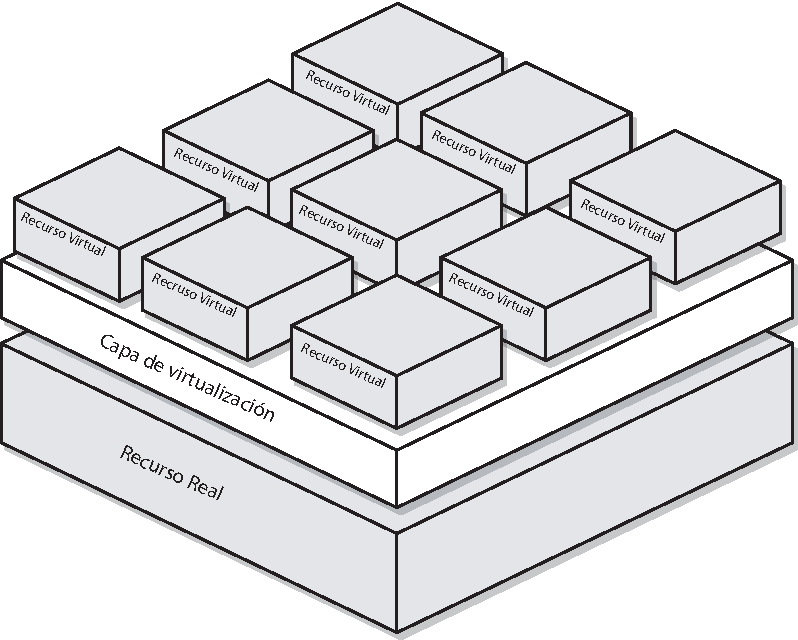
\includegraphics[width=8cm]{Pictures/divisionRecursosFisicosConV12N.pdf}
	\vspace{-0.2cm}
	\caption{División de recursos a través de la virtualización}
	\label{fig:divisionDeRecursosConVirtualizacion}
\end{figure}

Desafortunadamente la arquitectura de computadores x86 a pesar de ser una de las más populares en el mundo, no es virtualizable al 100\% \parencite{Adams}. En esta arquitectura, al ejecutar instrucciones en modo no privilegiado, algunas de ellas pueden fallar silenciosamente en lugar de provocar una trampa y así brindar su respectivo tratamiento. Esta situación ha tenido respuesta a través de mecanismos y formas de virtualización que actúan en diversos niveles de abstracción. Los niveles de abstracción dónde la virtualización tiene lugar son los siguientes: nivel del conjunto de instrucciones, nivel de abstracción de hardware, nivel de sistema operativo, nivel de interfaz de biblioteca de nivel de usuario y finalmente en el nivel de aplicación \parencite{Chiueh2005}.\\

Los conceptos acerca de la virtualización se presentan agrupados en las categorías \textit{elementos} y  \textit{técnicas de la virtualización}, cuya descripción se muestra en los apartados siguientes.


\subsection{Elementos de la virtualización}

Los elementos \textit{máquina real}, \textit{máquina virtual} y \textit{monitor de máquinas virtuales}, son considerados básicos para la comprensión de las tecnologías de virtualización y se describen a continuación.

\subsubsection{Máquina real}

El término \textit{máquina real} (RM por sus siglas en inglés \textit{Real Machine}) referencia los elementos físicos de la infraestructura tecnológica que conforman un computador; ya sea un computador personal, una estación de trabajo o un servidor. Otras referencias a este concepto son los términos en inglés \textit{hardware}, \textit{physical hardware}, \textit{bare-metal}. En el ámbito informático comercial es común que se refiera al concepto de RM utilizando la palabra \textit{anfitrión} o en inglés \textit{host} \parencite{VMware2008}. 

\subsubsection{Máquina virtual}

El concepto de \textit{máquina virtual} (VM por sus siglas en inglés \textit{Virtual Machine}) no es nuevo y fue formalizado en la tesis de  \textcite{Goldberg1973} y publicado en el trabajo académico de \textcite{Goldberg1974}; en estos trabajos se establecen las bases conceptuales para determinar el significado de una VM, siendo esta asumida como un duplicado eficiente y aislado de una RM, ver figura \ref{fig:TheVirtualMachineMonitor_Popek1974}.\\

Actualmente el concepto de VM hace referencia a un ambiente operativo para el conjunto de aplicaciones del nivel de usuario, lo cual incluye librerías, llamados al sistema, interfaces/servicios, configuraciones del sistema, procesos y archivos de estado \parencite{Chiueh2005}. Otra forma de presentar el concepto de VM según \textcite{Solis2014}, es relacionarlo con una capa de software, la cual se posiciona entre los recursos hardware o software y las aplicaciones. También es muy común que en el ámbito informático comercial se refiera al concepto de VM utilizando la palabra \textit{invitado(a)} o en inglés \textit{guest} \parencite{VMware2008}. Finalmente, \textcite{Pek2013} establecen que una VM, es también considerada como una abstracción de recursos de computación presentados como servicio para permitir que éstos operen simultáneamente sobre la misma infraestructura de la RM .

\begin{figure}[!hbtp]
	\centering
	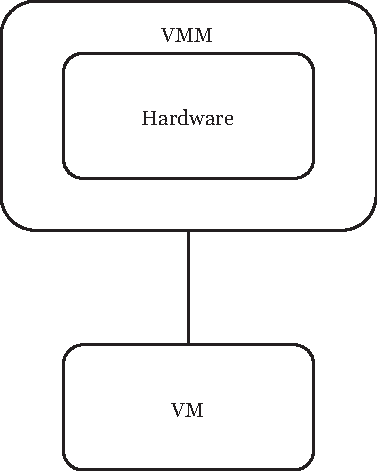
\includegraphics[width=5cm]{Pictures/VMMPopek1974.pdf}
	\vspace{-0.2cm}
	\caption{Visión general de MV y VMM por \textit{Popek} y \textit{Goldberg}.\footnotemark[2]{} }
	\label{fig:TheVirtualMachineMonitor_Popek1974}
\end{figure}

\footnotetext[2]{Basada en la figura original del monitor de máquina virtual del trabajo \textit{formal Requirements for Virtualizable Thrid Generation Architectures} de Gerald J. Popek y Robert P. Goldberg en 1974.}

\subsubsection{Monitor de máquinas virtuales}

El término monitor de máquina virtual (VMM por sus siglas en inglés \textit{Virtual Machine Monitor}), fue establecido en el trabajo de \textit{Popek} y \textit{Goldger} \cite{Popek1974}, en el cual  se definieron las bases conceptuales de un VMM como una pieza de software que tiene las siguientes tres características esenciales: 
\begin{enumerate}
	\item \textit{Equivalencia}: Proveer un ambiente para los programas, el cual es idéntico a la máquina original.\\
	
	\item \textit{Desempeño}: Los programas que se ejecutan en este ambiente muestran, en el peor de los casos, solo una degradación en velocidad.\\
	
	\item \textit{Control de recursos}: El VMM está en completo control de los recursos del sistema.\\ 
\end{enumerate}

La definición de un VMM está relacionada con una capa software que proporciona  infraestructura de soporte utilizando los recursos de un nivel más bajo (generalmente \textit{hardware}), para crear múltiples máquinas virtuales que son independientes y aisladas entre sí \parencite{Chiueh2005, Cafaro2011}. De manera similar, \textcite{Stallings2015}  determina  que un VMM, es un software que actúa como un intermediador entre la RM y las VMs; este software es comúnmente llamado \textit{hipervisor}, el cual permite que muchas máquinas virtuales coexistan de forma segura en una única RM. La cantidad de máquinas virtuales que existen en una sola máquina real, determina el índice de consolidación que para el caso particular de la figura \ref{fig:VMM}, es de 9 a 1 expresado como (9:1). Entre mayor sea el índice de consolidación mejor será el ROI y menos el TCO de la máquina real utilizada. Algunas de las funciones y responsabilidades de los hipervisores son la emulación, aislamiento, asignación de recursos y el encapsulamiento \parencite{Hoopes2009}.

\begin{figure}[!hbtp]
	\centering
	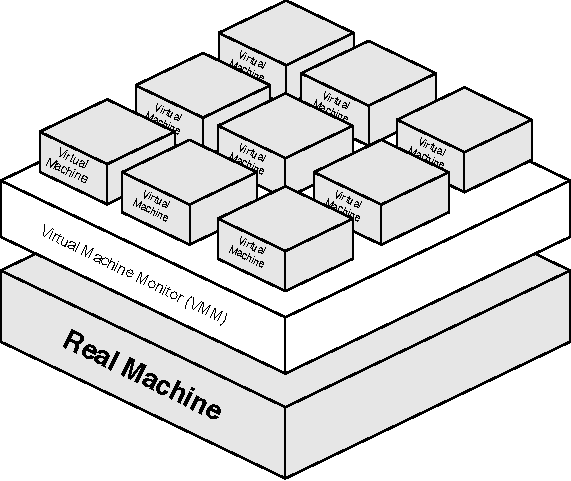
\includegraphics[width=8cm]{Pictures/VMMGeneric.pdf}
	\vspace{-0.2cm}
	\caption{Monitor de máquinas virtuales (VMM) o hipervisor}
	\label{fig:VMM}
\end{figure}

\subsection{Técnicas de virtualización}

A continuación, se describen dos de las principales técnicas de virtualización comúnmente utilizadas con son la \textit{basada en hipersivor} y la \textit{basada en contenedores}, estas técnicas permiten en general lograr consolidar componentes hardware y brindar un ambiente de ejecución virtual para sistemas o procesos respectivamente.

\subsubsection{Virtualización basada en hipervisor}

La técnica de virtualización basada en hipervisor consiste en la utilización del VMM como elemento central, el cual puede estar ubicado de dos maneras diferentes. La primera forma consiste en ubicar el hipervisor directamente sobre el hardware. Esta técnica es también conocida como virtualización \textit{bare-metal} o \textit{nativa}, y al hipervisor se le denomina de \textit{Tipo 1} (Figura \ref{fig:Bare-metalHypervisor}).  La utilización de este tipo de hipervisor no necesita la presencia de un sistema operativo subyacente en la RM. La segunda realiza la instalación del hipervisor sobre un sistema operativo existente. Esta técnica es también conocida como virtualización \textit{alojada} o \textit{basada en host}, y al hipervisor se le considera de \textit{Tipo 2} (ver figura \ref{fig:host-basedHypervisor}). Como característica general de la virtualización basada en hipervisor, se tiene la creación de máquinas virtuales completas, las cuales pueden ejecutar sistemas operativos \textit{guest} independientes y posiblemente diferentes, siempre y cuando sean compatibles con arquitectura virtual entregada. 


\begin{figure}[!hbtp]
	\centering
	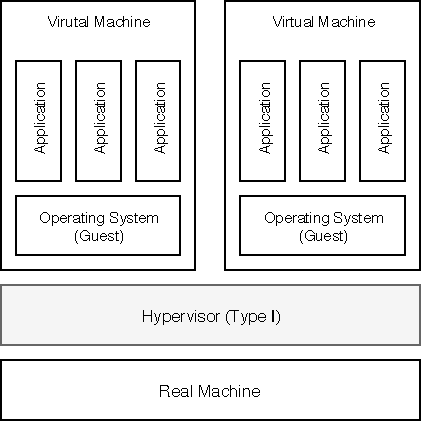
\includegraphics[width=8cm]{Pictures/bare-metalHypervisor.pdf}
	\vspace{-0.2cm}
	\caption{Bare-metal Hypervisor}
	\label{fig:Bare-metalHypervisor}
\end{figure}

\begin{figure}[ht] %[!hbtp]
	\centering
	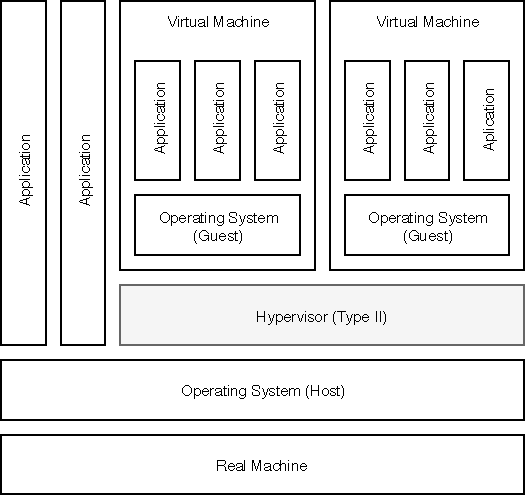
\includegraphics[width=8cm]{Pictures/host-basedHypervisor.pdf}
	\vspace{-0.2cm}
	\caption{Hoste based hypervisor}
	\label{fig:host-basedHypervisor}
\end{figure}

\subsubsection{Virtualización basada en contenedores}

La técnica de virtualización basada en contenedores utiliza como base un sistema operativo preexistente y consiste en la generación de entornos virtuales de ejecución para procesos. Estos entornos de ejecución son comúnmente llamados \textit{contenedores} (ver figura \ref{fig:container-baseVirtualization}). Esta técnica de virtualización gana cada día mayor aceptación en los ámbitos académico y productivo, debido a que, a diferencia de la virtualización basada en hipervisor, no es necesario generar VMs con sistemas operativos completos, sino que se utilizan partes fundamentales del sistema operativo \textit{host} para generar los entornos virtuales de operación para los procesos \parencite{Kon2017}. Lo anterior supone una menor carga computacional necesaria para generar el entorno virtual y de igual forma supone que dicho entorno está sujeto al tipo de sistema operativo subyacente. 


\begin{figure}[ht] % [!hbtp]
	\centering
	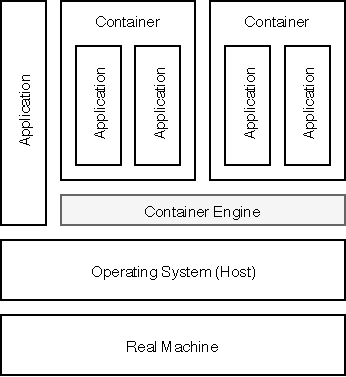
\includegraphics[width=8cm]{Pictures/container-baseVirtualization.pdf}
	\vspace{-0.2cm}
	\caption{Container-based virtualization}
	\label{fig:container-baseVirtualization}
\end{figure}


\subsection{Taxonomía de Tecnologías de Virtualización}



\begin{figure}[!htp]
	\centering
	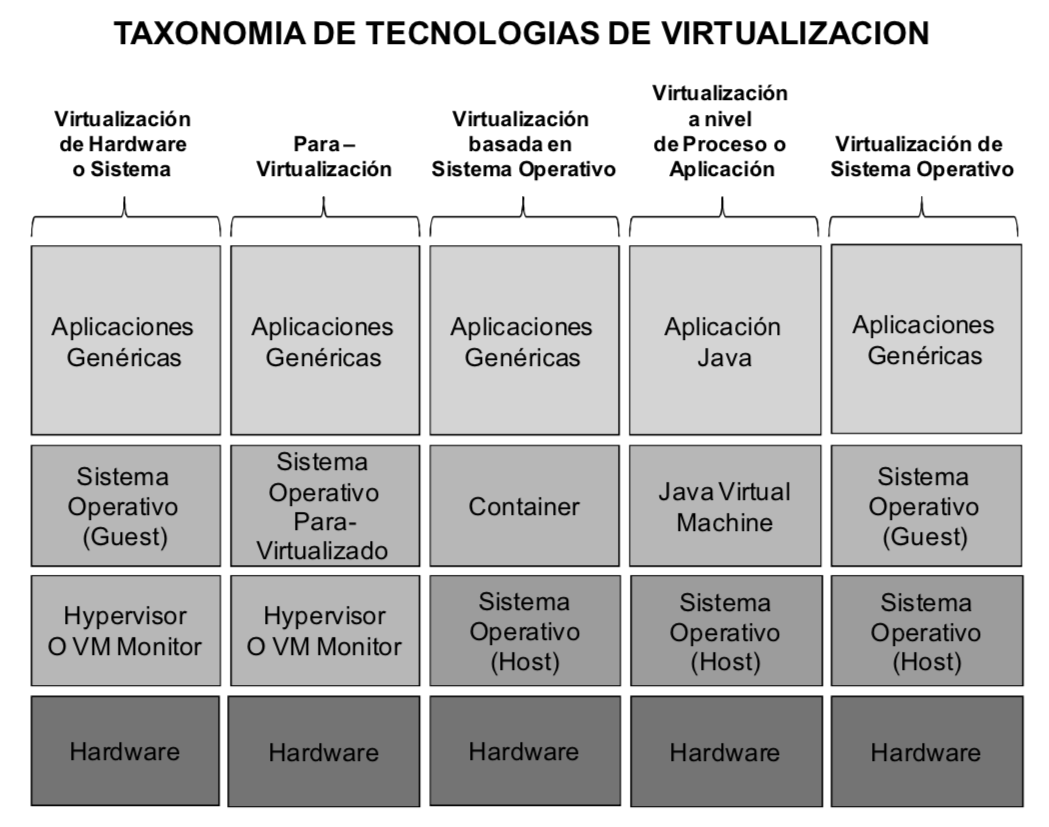
\includegraphics[width=0.8 \linewidth]{Pictures/taxonomiaPessolani.png}
	\vspace{-0.2cm}
	\caption{Taxonomía de máquinas virtuales propuesta por Pessolani y otros en 2012\footnotemark[8]{}}
	\label{fig:taxonomiaPessolani}
\end{figure}

\footnotetext[8]{Figura basada en el trabajo \textit{Sistema de virtualización con recursos distribuidos } de Pablo Pessolani, Toni Cortes, Silvio Gonnet y Fernando Tinetti, en 2005.}

El presente trabajo utiliza como base conceptual la taxonomía de tecnologías de virtualización propuesta por \textcite{Pessolani2012}. Esta taxonomía posee cinco categorías principales como son:\textit{virtualización de hardware o sistema}, \textit{para-virtualización}, \textit{virtualización basada en sistema operativo}, \textit{virtualización a nivel de proceso o aplicación} y finalmente \textit{virtualización de sistema operativo}. (Ver figura \ref{fig:taxonomiaPessolani}). Adicionalmente, también se muestran capas por cada categoría, las cuales sugieren un nivel en el cuál tiene lugar cada tipo de virtualización. A continuación, se describen las categorías de esta taxonomía:\\


\subsubsection{Virtualización de Hardware o Sistema}
Esta categoría se caracteriza por utilizar un hipervisor \textit{Tipo 1} directamente sobre el hardware (\textit{bare-metal}) y a partir de él, se ubican las VMs con sus respectivos sistemas operativos \textit{guest} (estos sistemas no logran percibir la condición de virtualización), los cuales soportan a su vez las aplicaciones particulares de los usuarios \parencite{Pessolani2012}.\\

Esta técnica de virtualización es también llamada \textit{Virtualización completa} y con relación a la arquitectura x86, está basada en la combinación de técnicas de traducción binaria y ejecución directa. Este enfoque busca traducir el código del kernel del sistema operativo \textit{guest}, para reemplazar las instrucciones no virutalizables con unas nuevas que tengan efecto en el hardware virtual\parencite{VMware2008}. 

\subsubsection{Para-Virtualización}
Esta categoría tiene la distribución de sus elementos similar a la \textit{virtualización de hardware o sistema} y también utiliza un hipervisor \textit{Tipo 1}, pero en este caso el sistema operativo \textit{guest} se considera que está \textit{Para-virtualizado}, esto es que ha sido modificado para tener conocimiento del hecho de estar virtualizado y de esta manera sacar provecho de esa situación y en consecuencia obtener un mejor rendimiento. \parencite{Pessolani2012}\\

La palabra ``Para'' viene del Griego y significa ``al lado de''. En este contexto entonces signfica ``al lado de la virtualización''. La \textit{paravirtualización} se refiere a la comunicación entre el sistema operativo \textit{guest} y el hipervisor para mejorar el desempeño y la eficiencia. Esta técnica de virtualización también es conocida como \textit{Virtualización asistida por el sistema operativo} \parencite{VMware2008}.



\subsubsection{Virtualización basada en Sistema Operativo}
Esta categoría, a diferencia de las anteriores no utiliza un hipervisor y en contraste, se basa en la utilización de espacios de trabajo independientes llamados \textit{contenedores}, los cuales están basados en el sistema operativo \textit{host}. Estos contenedores permiten la ejecución de aplicaciones genéricas de forma independiente.\\

\subsubsection{Virtualización a nivel de proceso o Aplicación}
Este tipo de virtualización utiliza un proceso  o aplicación sobre el sistema operativo para brindar una máquina virtual que permita la ejecución de procesos basados en esa máquina, por ejemplo JVM y las aplicaciones Java respectivamente. \\ 

\subsubsection{Virtualización de Sistema Operativo}
Este tipo de virtualización necesita un sistema operativo \textit{host} el cual lleva a cabo las funciones de un hipervisor para soportar los sistemas operativos \textit{guests},  que a su vez tienen sus propias aplicaciones completamente independientes, por ejemplo \textit{User Mode Linux} \parencite{Dike2006}  y \textit{Minix Over Linux} \parencite{Pessolani2012}.

% Sección: Contexto Histórico de la virtualización	
\section{Contexto histórico de las tecnologías de virtualización} \label{historia}

Se puede considerar que la idea relacionada con la virtualización tiene sus inicios desde los comienzos mismos de la computación. Una de las principales motivaciones que dieron origen al concepto de virtualización fue encontrar una manera para aprovechar los recursos de computación existentes y así compartirlos de la manera más eficientemente posible entre diversas tareas. \\

Particularmente, la virtualización tiene sus inicios en la década de 1960, especialmente con el aporte del personal del MIT (Massachusetts Intitute of Technology), quienes reconocieron la necesidad de máquinas virtuales \parencite{ Varian1997, Ameen2013}.\\ 

Para la década de 1970, IBM desarrolló el sistema VM/370, este dispositivo permitía a cada usuario ejecutar acciones como si estuvieran en un entorno aislado, pero todo dentro de un entorno informático de tiempo compartido \parencite{Douglis2013, Varian1997}. En esta misma década \textcite{Goldberg1973} determino en su tesis el concepto de máquina virtual y lo publico junto con \textit{Gerald Popek} en el trabajo  denominado \textit{Formal requirements for virtualizable third generation architectures} \parencite{Popek1974}.\\


Para la década de 1980 y mediados de 1990, \textcite{Varasteh2017,Agrawal2013} señalan que la virtualización perdió popularidad gracias a la disminución de los costos en la fabricación de los servidores y la proliferación de las computadoras personales. Esta situación facilitó a las empresas la implantación de un modelo de trabajo distribuido con respecto al hardware y la  adquisición de máquinas independiente para cada necesidad. Por ejemplo, para los servicios Web, bases de datos, correo electrónico, servicio de directorio y el alojamiento de las aplicaciones proprias de cada negocio. Con el pasar los años, esta forma de trabajo distribuido también trajo consigo mayores problemas en la administración de los recursos hardware y el incremento del costo total de propiedad por el aumento del consumo de energía para operar los centros de procesamiento de datos. Por otro lado, \textcite{Ranjith2017} determinan que este tipo de situaciones también presentan una tendencia poco amigable con el medio ambiente. \\

Para finales de los 90s y considerando la problemática anteriormente descrita, la virtualización vuelve nuevamente a ganar  aceptación como una solución complementaria para lograr la consolidación en los centros de procesamiento de datos \parencite{Oludele2014, Sukmana2016}.\\

Con el propósito de identificar algunos de los hitos más representativos en el contexto histórico de la virtualización, a continuación se presenta una línea de tiempo basada en el trabajo de \textcite{Marshall2006}:\\
				
\textbf{1960}\\
\begin{itemize}
	\item Identificación de la necesidad de virtualización.  \parencite{Ameen2013}.\\
	\item IBM introduce el concepto de sistema de tiempo compatido (TSS por la sigla en inglés de \textit{Time Sharing Systems}) \parencite{Dittner2011}.\\
\end{itemize}				
				
\textbf{1964}\\
\begin{itemize}
	\item IBM anuncia el lanzamiento de la máquina \textit{IBM System/360}.\\
	
	\item Lanzamiento del programa CP-40. (CP por la sigla en inglés de \textit{Control Program}) por parte del Centro Científico Cambridge de IBM (SCS por las sigla en inglés de \textit{Cambridge Scientific Center}).\\
\end{itemize}

\textbf{1965}\\
\begin{itemize}
	\item IBM anuncia el lanzamiento de la máquina \textit{IBM System/360 modelo 67 con TSS}.\\
\end{itemize}

\textbf{1967}\\
\begin{itemize}
	\item CP-40 y CMS (\textit{Program/Cambridge Monitor System}).\\
\end{itemize}

\textbf{1968}\\
\begin{itemize}
	\item CP-67 versión 1.\\
\end{itemize}

\textbf{1969}\\
\begin{itemize}
	\item CP-67 versión 2.\\
\end{itemize}

\textbf{1970}\\
\begin{itemize}
	\item CP-67 versión 3.\\
\end{itemize}

\textbf{1971}\\
\begin{itemize}
	\item CP-67 versión 3.1.\\
\end{itemize}

\textbf{1972}\\
\begin{itemize}
	\item IBM System/360 Advanced Function.\\
\end{itemize}

\textbf{1973}\\
\begin{itemize}
	\item Fundación de la asociación metropolitana de usuarios de máquinas virtuales de New York (MVMUA por la sigla en inglés \textit{Metropolitan VM User Association}).\\
	
	\item \textit{Robert Goldberg} publica el trabajo llamado \textit{Architectural Principles for Virtual Computer Systems} \parencite{Goldberg1973}.\\
	
\end{itemize}

\textbf{1974}\\
\begin{itemize}
	\item VM/370 Release 2.\\
	
	\item \textit{Robert Goldberg} publica el trabajo llamado \textit{Survey of virutal machines research} \parencite{Goldberg1974}.\\
	
	\item \textit{Poket} y \textit{Goldberg} publican el trabajo llamado \textit{Formal requirements for virtualizable third generation architecture} \parencite{Popek1974}\\.
\end{itemize}


\textbf{1980}\\
\begin{itemize}
	\item Introducción de la virtualización a nivel de lenguaje.\\
	
	\item Se introdujo la \textit{virtualización a nivel de lenguaje} para permitir la potabilidad y el aislamiento a nivel de la aplicación\parencite{Douglis2013}. \\ 
\end{itemize}

\textbf{1987}\\
\begin{itemize}
	\item Debido al surgimiento de Internet, se dio la necesidad de incorporar el soporte para TCP/IP en las máquinas virtuales conocido como VM TCP/IP.\\
\end{itemize}

\textbf{1988}\\
\begin{itemize}
	\item \textit{Jon Garber} crea \textit{Connextix},  una empresas dedicada a la virtualización.\\
\end{itemize}


\textbf{1991}\\
\begin{itemize}
	\item CMS Multi-Tasking.\\
	
	\item P/370 \\.
\end{itemize}


\textbf{1996}\\
\begin{itemize}
	\item Introducción de la máquina virtual de Java (JVM por la sigla \textit{Java Virtual Machine}) \parencite{Lindholm1997,Douglis2013}. \\
\end{itemize}


\textbf{1997}\\
\begin{itemize}
	\item La empresa Connectix libera \textit{Virtual PC 1.0} para la plataforma Macinthosh. \\
\end{itemize}
				
\textbf{1998}\\
\begin{itemize}
	\item \textit{Diane Greene} funda a \textit{VMware Inc},  una empresas dedicada a la virtualización para los computadores con arquitectura x86.\\
\end{itemize}
				
\textbf{1999}\\
\begin{itemize}
	\item VMware lanza \textit{VMware Workstation 1.0}.\\
\end{itemize}
				
\textbf{2000}\\
\begin{itemize}
	\item VMware lanza \textit{VMware GSX Server (hosted)} para Windows y Linux.\\
	
	\item \textit{FreeBSD Jails} como una implementación inicial en \textit{FreeBSD 4.0}.\\
\end{itemize}
				
\textbf{2001}
\begin{itemize}
	\item VMware lanza 
	
	\begin{itemize}
		\item \textit{VMware ESX Server 1.0 (hosteless)}. Esta versión, no requiere un sistema operativo subyacente sobre el hardware; esta técnica de instalación es también conocida como \textit{bare-metal}. \\

		\item \textit{VMware Workstation 3.0}\\
	\end{itemize}
	
	\item Conneectix lanza \textit{Virtual PC for Windows}.  \\
	
	\item Linux VServer\\
	
\end{itemize}
				
\textbf{2002}
\begin{itemize}
	\item VMware lanza: \\
	\begin{itemize}
		\item \textit{VMware GSX Server 2.0}\\
		\item \textit{VMware ESX 1.5}\\
		\item \textit{VMware Workstation 3.1}\\
	\end{itemize}
	
	 \item Los productos de VMware ya cuenta con más de un millón de usuarios. \\
\end{itemize}

\textbf{2003}
\begin{itemize}
	\item VMware lanza: \\
	\begin{itemize}
		\item \textit{VMware GSX Server 2.5}.\\
		\item \textit{VMware ESX 2.0}.\\
		\item \textit{VMware Virtual Center}.\\
		\item \textit{VMware vMotion}.\\
		\item \textit{VMware Virtual SMP}.\\
		\item \textit{VMware Workstation 4.0}\\
	\end{itemize}
	\item Connectix lanza \textit{Virtual Server 1.0 RC}.\\
	
	\item Microsoft adquiere la empresa Connectix con los productos \textit{Virutal PC} y \textit{Virtual Server}. \\
	
\end{itemize}
			
\textbf{2004}
\begin{itemize}
	\item La empresa EMC Inc adquiere a VMware Inc.\\
	
	\item VMware lanza: \\
	\begin{itemize}
		\item Soporte para 64-bits\\ 
		\item \textit{VMware GSX Server 3.0 y 3.1}\\
		\item \textit{VMware ESX Server 2.5}\\
		\item \textit{VMware Workstation 4.5}\\
		
		
	\end{itemize}

	\item Xen v1 Linux con Paravirtualization. \\
	\item Microsoft lanza \textit{Microsoft Virtual Server 2005}. \\
	
\end{itemize}

\textbf{2005}
\begin{itemize}
	\item VMware lanza los siguientes productos: \\
	
	\item \textit{VMware Workstation 5.0 y 5.5}\\
	
	\item \textit{VMware Player}\\
	
	\item Xen v2 Linux con Paravirtualization\\
	
	\item \textit{Solaris Zones} incluidas en el sistema operativo \textit{Solaris}\\
	
	\item OpenVZ (Open Virtuozzo)\\
\end{itemize}

\textbf{2006}
\begin{itemize}
	\item \textit{VMware Server} \\
	
	\item Microsoft lanza \textit{Virtual Server 2005 R2 Enterprise Edition}\\
	
	\item \textit{Virtual Server 2005 R2 Enterprise Edition SP1} incluye soporte para las tecnologías de virtualización asistida por hardware de Intel VT (IVT) y AMD Virtualization (AMD-V)\\
	
	\item La empresa Parallels Inc lanza \textit{Parallels Workstation for Mac OS X}\\
	
	\item Google lanza \textit{Process Containers} \\
	
\end{itemize}
	
\textbf{2007}\\
\begin{itemize}
	\item Primera generación de \textit{Hardware Assisted Virtualization}\\
	
	\item KVM es integrado con el Kernel Linux\\
	
	\item \textit{Innotek GmbH } lanza \textit{Virtual Box (Open Source Ediction)}\\
	
	\item Xen v3 Linux con  \textit{Hardware Assisted Virtualization}\\
	
	\item Solaris Containers sólo para arquitectura SPARC\\
	
	\item \textit{VMware Workstation 6.0}\\
	
	\item \textit{Parallel Desktop 3.0 for Mac}\\
\end{itemize}
			
\textbf{2008}\\
\begin{itemize}
	\item \textit{VMware Workstation 6.5}\\
	
	\item Sun Microsystems aquiere a \textit{Innotek}\\
	
	\item Microsoft lanza \textit{Hyper-V} junto con \textit{Windows Server 2008} como un rol del sistema operativo\\
	
	\item Linux Containers (LXC)\\
	
	\item Linux VServer\\
	
	\item \textit{Parallel Desktop 4.0 for Mac}\\
\end{itemize}
			
\textbf{2009}\\
\begin{itemize}
	\item Microsoft lanza \textit{Windows Virtual PC} \\
	
	\item Hyper-V Server 2008 R2\\
	
	\item \textit{VMware Workstation 7.0}\\
	
	\item \textit{Parallel Desktop 5.0 y 6.0 for Mac}\\
\end{itemize}

\textbf{2010}\\
\begin{itemize}
	\item \textit{Parallel Desktop 6.0 for Mac}\\	
\end{itemize}

\textbf{2011}\\
\begin{itemize}
	\item \textit{VMware Workstation 8.0}\\
	
	\item Oracle Corporation aquiere a Sun Microsystems renombra \textit{Virtualbox} como \textit{Oracle VM VirtualBox}\\
	
	\item \textit{Parallel Desktop 7.0 for Mac}\\	
\end{itemize}

\textbf{2012}\\
\begin{itemize}
	\item \textit{VMware Workstation 9.0}\\
	
	\item \textit{Parallel Desktop 8.0 for Mac}\\	
\end{itemize}

\textbf{2013}\\

\begin{itemize}
	\item Google inicia a trabaja en \textit{LMCTFY} (por la sigla en ingles \textit{Let Met Contain That For You})\\
	
	\item Lanzamiento de \textit{Docker}, desarrollado por \textit{Salomón Hykes}. Docker inicialmente utiliza la interfaz LXC para acceder a las capacidades de virtualización del kernel Linux \parencite{Turnbull2014}.  Se libera hasta la versión 0.7.2\\
	
	\item \textit{VMware Workstation 10.0}\\
	
	\item \textit{Parallel Desktop 9.0 for Mac}\\	
	
\end{itemize}

\textbf{2014}\\
\begin{itemize}
	\item Lanzamiento de \textit{Docker} 0.9, el cual utiliza una librería propia como interfaz para remplazar a LXC llamada \textit{libcontainer} y así acceder a las capacidades del kernel directamente \parencite{Kurtzer2017}\\
	
	\item \textit{Parallel Desktop 10.0 for Mac}\\	
	
	\item \textit{Docker} desde la versión 0.7.3 hasta la 1.4.1
	
\end{itemize}


\textbf{2015}\\
\begin{itemize}
	\item La empresa \textit{Dell Inc} adquiere a EMC que en el 2004 había adquirido a VMware\\
	
	\item \textit{VMware Workstation 11.0 y 12.0}\\
	
	\item \textit{Parallel Desktop 11.0 for Mac}\\	
	
	\item Inicio del proyecto open-souce \textit{Singularity}. Una herramienta de virtualización a nivel del sistema operativo\\
	
	\textit{Docker} desde la versión 1.5.0 hasta la 1.9.1\\
	
\end{itemize}


\textbf{2016}\\
\begin{itemize}
	\item \textit{Parallel Desktop 12.0 for Mac}\\	
	\item \textit{Singularity 1.0 a 2.2}\\
	
	\textit{Docker} desde la versión 1.10.0 hasta la 1.12.5\\	
\end{itemize}

\textbf{2017}\\
\begin{itemize}
	\item \textit{VMware Workstation 14.0}\\
	\item \textit{Parallel Desktop 13.0 for Mac}\\	
	
	\textit{Docker} desde la versión 1.12.6 hasta la 1.13.1. Posteriormente, \textit{Docker} cambia la forma de realizar la numeración en la versión, para hacerla coincidir con el año y mes de liberación. También se agrega CE o EE para diferenciar la versión \textit{Community Edition} o \textit{Enterprise Edition} respectivamente. Para 2017 se entregaron desde la versión 17.03.0-ce hasta la 17.12.0-ce \parencite{DockerRelease2018}.\\
	
	\item \textit{Singularity 2.2.1 a 2.4}	\\
\end{itemize}

\textbf{2018}\\
\begin{itemize}
	\item \textit{VMware Workstation 15.0}\\
	\item \textit{Parallel Desktop 14.0 for Mac}\\		
	\item \textit{Docker 18.0.1-ce a 18.09.0-ce} \\
	\item \textit{Singularity 2.4.2 a 2.5.2} \parencite{Singularity2018}\\
\end{itemize}


\section{Ámbitos de aplicación de las tecnologías de virtualización} \label{ambitos}

Las tecnologías de virtualización tiene cabida en diversos ámbitos como la industria, la academia y la investigación. 

  de aplicación debido debido a los beneficios que presentan respecto a menor TCO y mejor ROI. 



\subsection{Ámbito Industrial}

\begin{description}
	\item[Centro de procesamiento de datos] Empresas especializadas en infraestructura con centro de procesaminto de datos (CDP o en inglés \textit{Datacenter}).
\end{description}



Facilita la aplicación de los planes de continuidad de negocio en las organizaciones. 

Desarrollo de software

Favorece el rápido despliegue de ambientes de trabajo, reduciendo así el tiempo de entrada en producción de nuevos empleados en las organizaciones. \\


Internet de las Cosas o IoT (por las siglas en inglés Internet Of Things) es una área que se está logrando potenciar gracias a la virtualización basada en el sistema operativo, también llamada \textit{Virtualización Liviana} (en inglés Lightwiht Virtualization). 



\subsection{Académico}

Enseñanza de las tecnologías de virtualización


Virtualización de entornos de trabajo (docker)


Lenguajes de programación (Java Virtual Machine y .NET)


\section{Identificación de herramientas de virtualización} \label{herramientas}





\chapter{Recursos Educativos}
Nota: ``Construir dos recursos educativos por cada tecnología de virtualización (seis en total) que a modo de ejemplo sirvan para ilustrar la implementación de una herramienta de virtualización'' 

\section{Recursos Educativos para la Virtualización de Hardware o Sistema}

\subsection{Recurso Educativo para la herramienta VMware ESXi}
\subsubsection{Propósito}

\subsubsection{Arquitectura}

\subsubsection{Aspectos técnicos generales}

Se debe aclarar que \textbf{VMWare ESXi} es software privativo, se debe adquirir una licencia para poder utilizarlo comercialmente. Para el presente trabajo se utilizan versiones de prueba de la herramienta. También es importante tener presente que para poder acceder a dichas versiones es necesario crear previamente una cuenta de usuario gratuita en el sitio web de VMWare (Ver figura \ref{fig:VMwareInstalacion01}).\\

\begin{figure}[!hbtp]
	\centering
	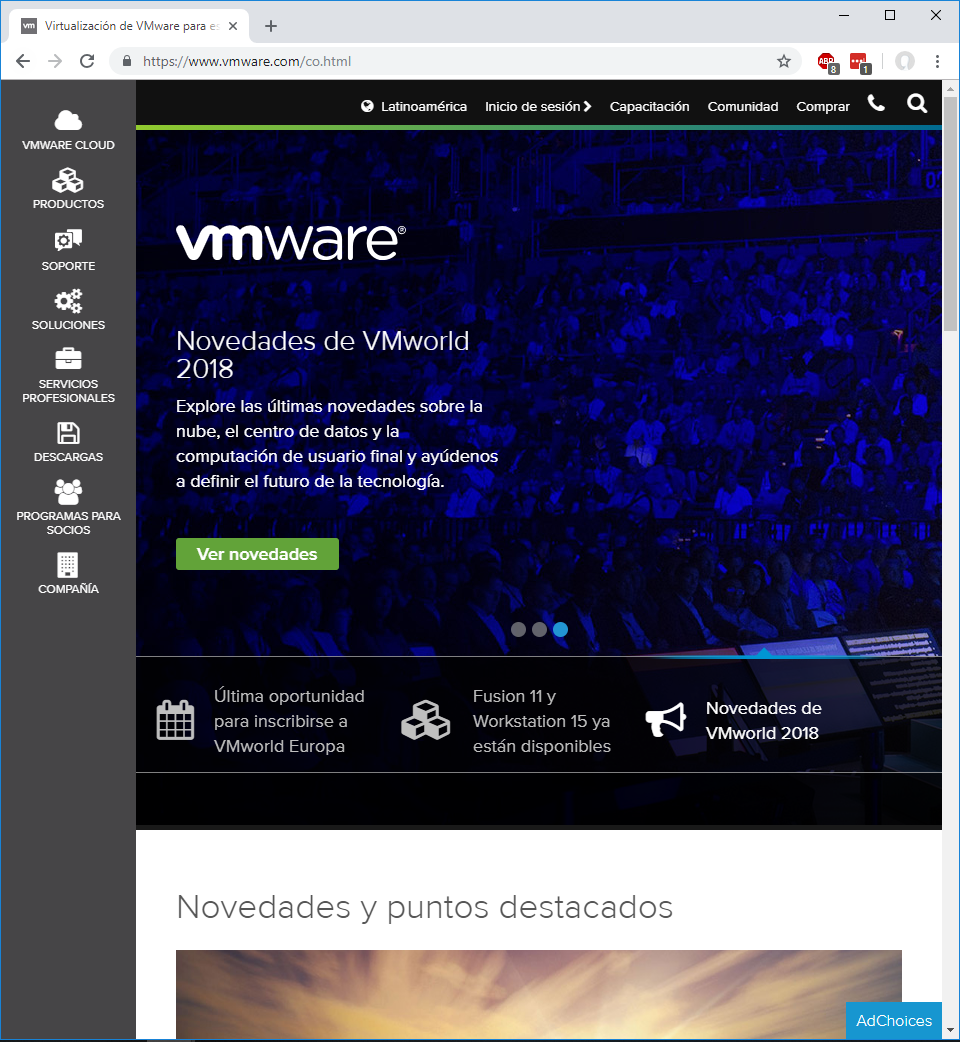
\includegraphics[width=\linewidth]{Trabajo/RecursosEducativos/RE01_VMwareESXi/RE_VMwareInstalacion01.png}
	\vspace{-0.2cm}
	\caption{Sitio web WMWare \url{www.vmware.com}.\footnotemark[2]{}}
	\label{fig:VMwareInstalacion01}
\end{figure}

\footnotetext[2]{La imagen corresponde a la captura de pantalla del sitio web \url{www.vmware.com}.}


\subsubsection{Instalación de VMware ESXi}

Para la instalación de VMWare ESXi es necesario tener la imagen del hipervisor, la cual puede ser obtenido desde la página oficial de VMWare, En la imagen se puede observar que se pueden descargar las diferentes versiones del VMWare ESXi, en el presente trabajo se trabaja con la versión 6.7.
Para la instalación se utilizó una máquina virtual con 8 GB de memoria RAM, un procesador Intel Core i7 6700-HQ y un disco duro de 100GB. Se debe tener la imagen en una memoria flash booteable o en un DVD. Al iniciar el sistema se debe seleccionar el arranque desde la memoria o el DVD y seleccionar como medio el SO VMWare ESXi como se puede observar en la figura \ref{fig:VMwareInstalacion02}.

\begin{figure}[!hbtp]
	\centering
	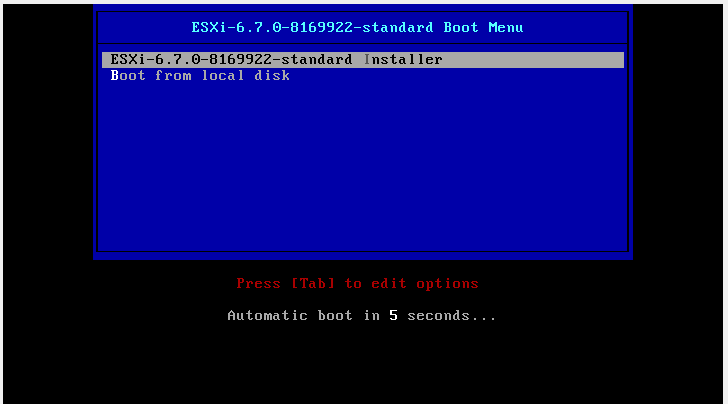
\includegraphics[width=\linewidth]{Trabajo/RecursosEducativos/RE01_VMwareESXi/RE_VMwareInstalacion02.png}
	\vspace{-0.2cm}
	\caption{Sitio Web WMWare \url{www.vmware.com}.\footnotemark[2]{} }
	\label{fig:VMwareInstalacion02}
\end{figure}

El sistema operativo comienza su carga en la memoria, tal como se ve en la imagen.


\begin{figure}[!hbtp]
	\centering
	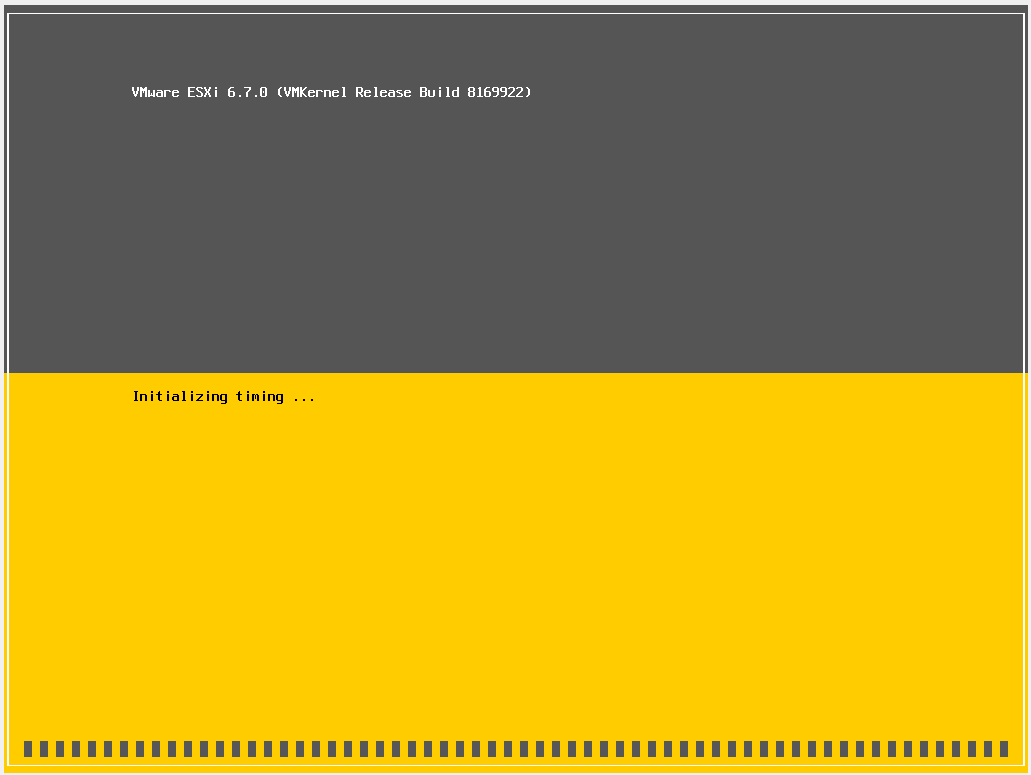
\includegraphics[width=\linewidth]{Trabajo/RecursosEducativos/RE01_VMwareESXi/RE_VMwareInstalacion03.png}
	\vspace{-0.2cm}
	\caption{Sitio Web WMWare \url{www.vmware.com}.\footnotemark[2]{} }
	\label{fig:VMwareInstalacion03}
\end{figure}

\begin{figure}[!hbtp]
	\centering
	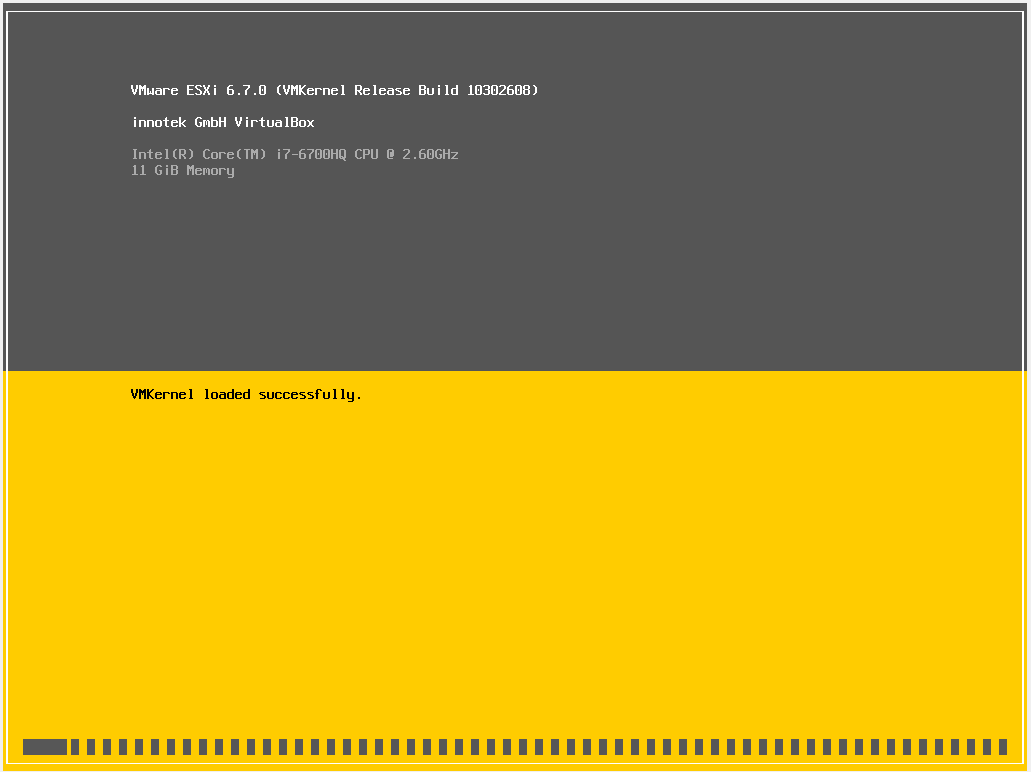
\includegraphics[width=\linewidth]{Trabajo/RecursosEducativos/RE01_VMwareESXi/RE_VMwareInstalacion04.png}
	\vspace{-0.2cm}
	\caption{Sitio Web WMWare \url{www.vmware.com}.\footnotemark[2]{} }
	\label{fig:VMwareInstalacion04}
\end{figure}

\begin{figure}[!hbtp]
	\centering
	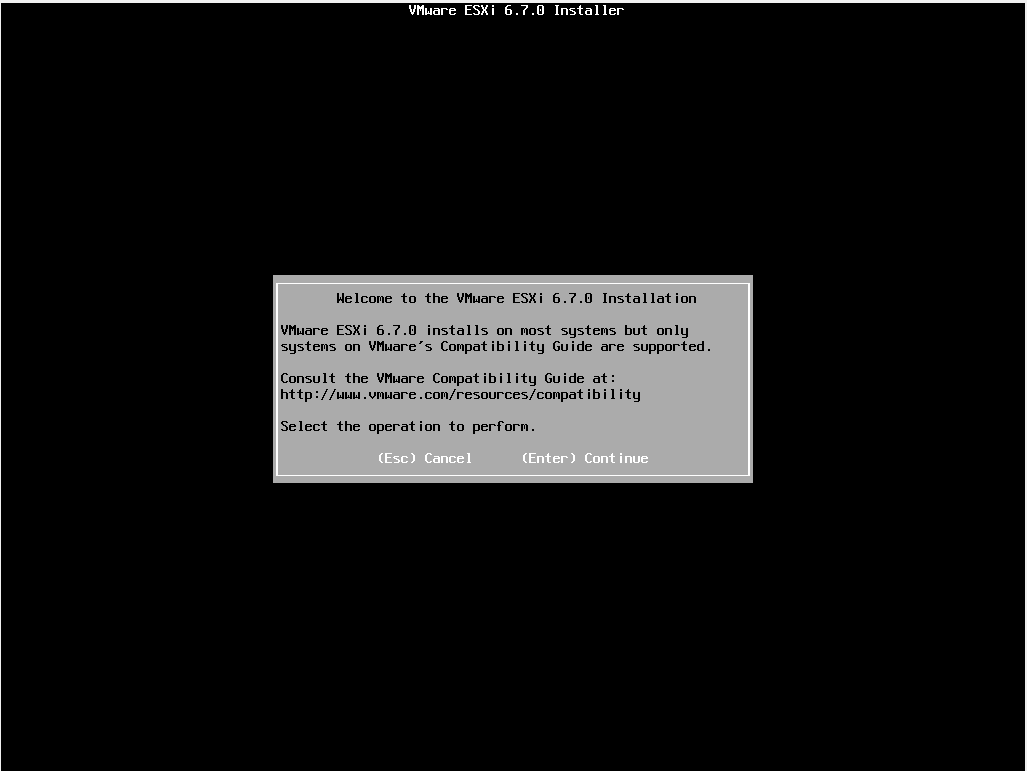
\includegraphics[width=\linewidth]{Trabajo/RecursosEducativos/RE01_VMwareESXi/RE_VMwareInstalacion05.png}
	\vspace{-0.2cm}
	\caption{Sitio Web WMWare \url{www.vmware.com}.\footnotemark[2]{} }
	\label{fig:VMwareInstalacion05}
\end{figure}

\begin{figure}[!hbtp]
	\centering
	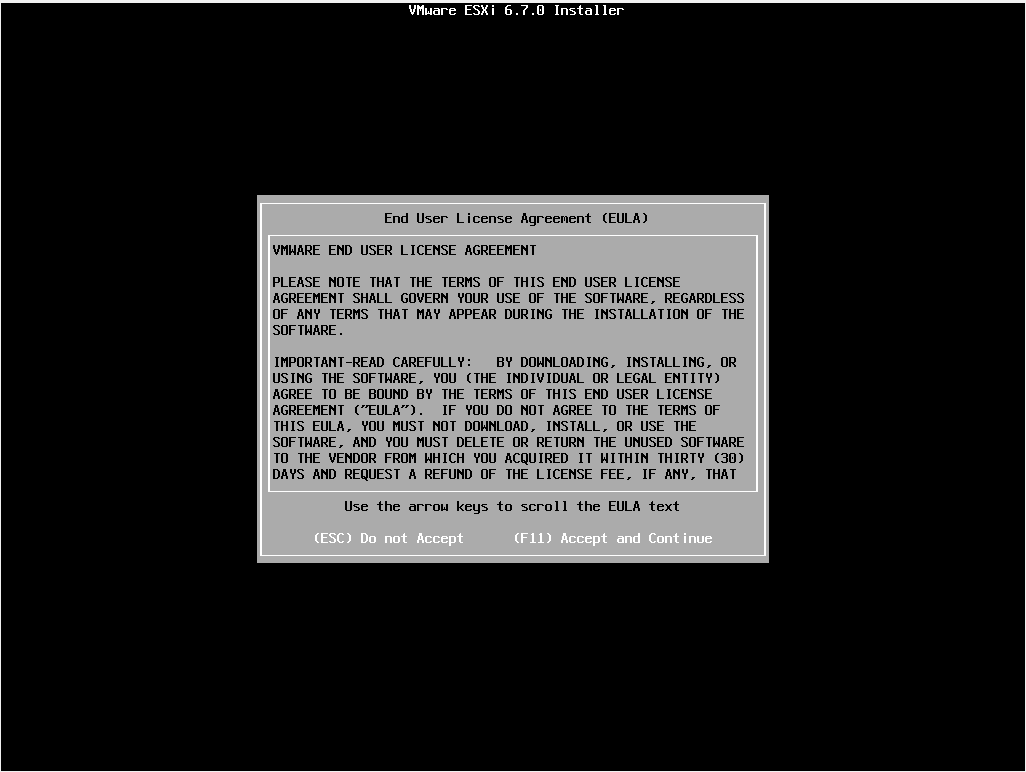
\includegraphics[width=\linewidth]{Trabajo/RecursosEducativos/RE01_VMwareESXi/RE_VMwareInstalacion06.png}
	\vspace{-0.2cm}
	\caption{Sitio Web WMWare \url{www.vmware.com}.\footnotemark[2]{} }
	\label{fig:VMwareInstalacion06}
\end{figure}


\begin{figure}[!hbtp]
	\centering
	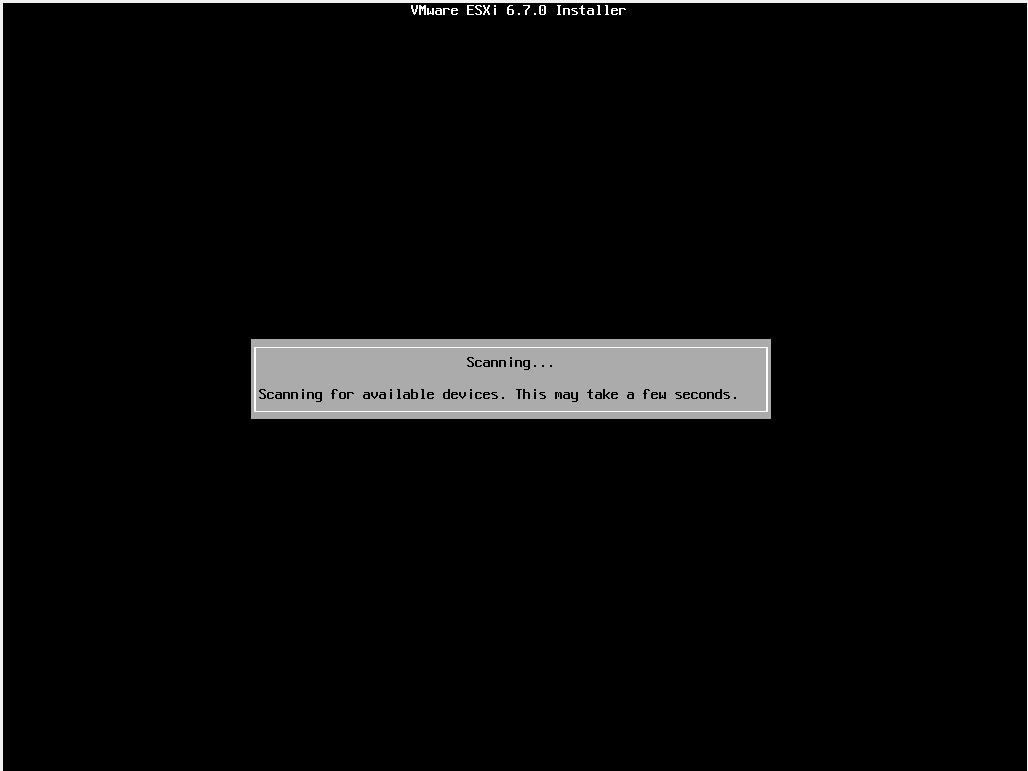
\includegraphics[width=\linewidth]{Trabajo/RecursosEducativos/RE01_VMwareESXi/RE_VMwareInstalacion07.png}
	\vspace{-0.2cm}
	\caption{Sitio Web WMWare \url{www.vmware.com}.\footnotemark[2]{} }
	\label{fig:VMwareInstalacion07}
\end{figure}


\begin{figure}[!hbtp]
	\centering
	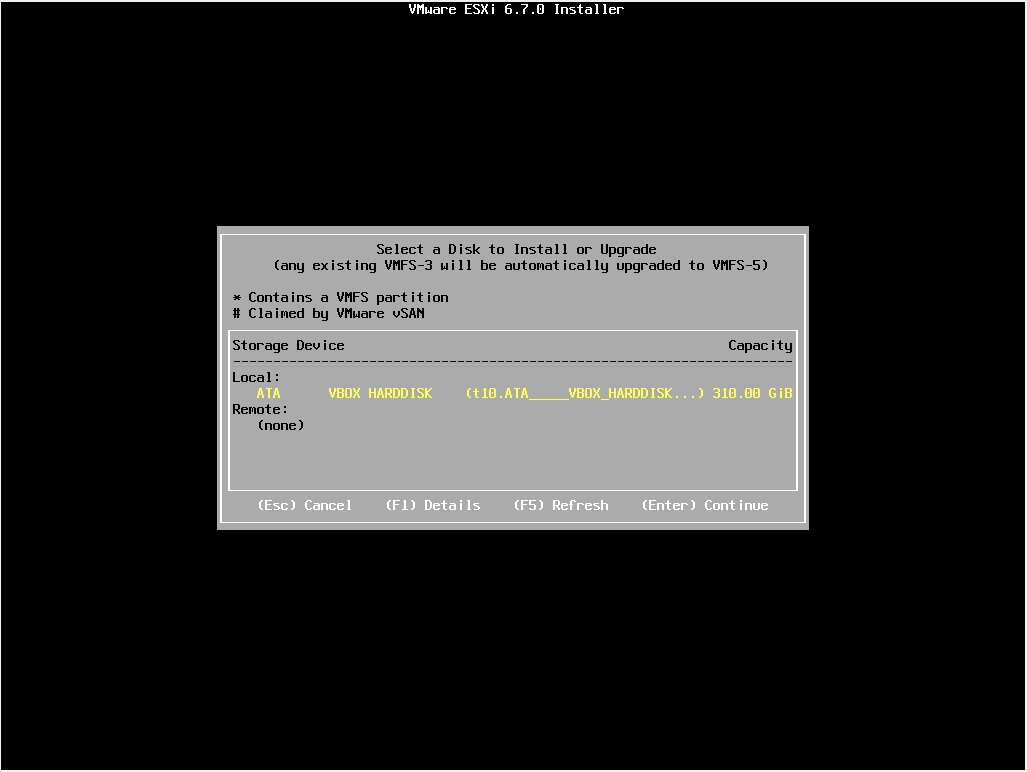
\includegraphics[width=\linewidth]{Trabajo/RecursosEducativos/RE01_VMwareESXi/RE_VMwareInstalacion08.png}
	\vspace{-0.2cm}
	\caption{Sitio Web WMWare \url{www.vmware.com}.\footnotemark[2]{} }
	\label{fig:VMwareInstalacion08}
\end{figure}


\begin{figure}[!hbtp]
	\centering
	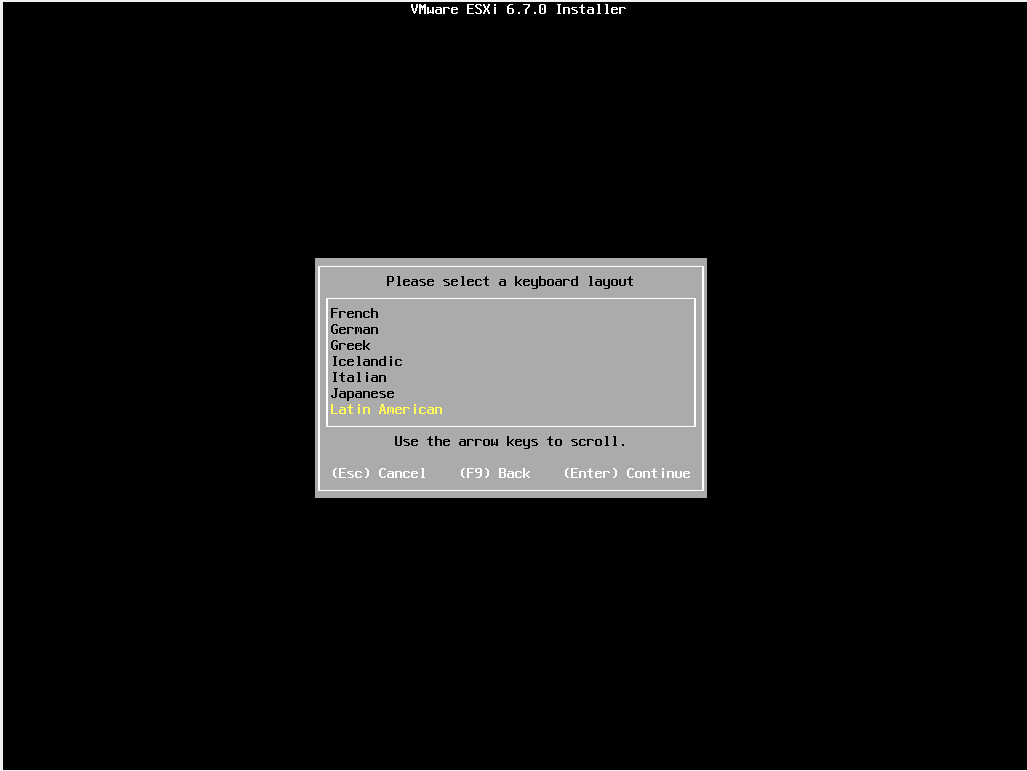
\includegraphics[width=\linewidth]{Trabajo/RecursosEducativos/RE01_VMwareESXi/RE_VMwareInstalacion09.png}
	\vspace{-0.2cm}
	\caption{Sitio Web WMWare \url{www.vmware.com}.\footnotemark[2]{} }
	\label{fig:VMwareInstalacion09}
\end{figure}


\begin{figure}[!hbtp]
	\centering
	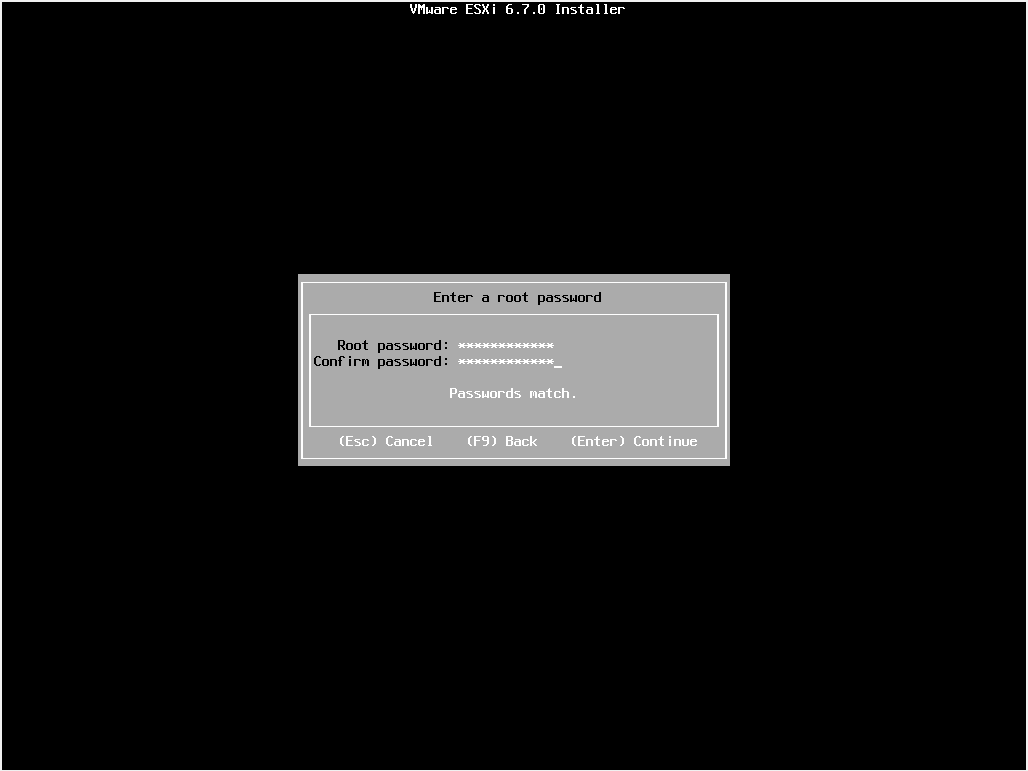
\includegraphics[width=\linewidth]{Trabajo/RecursosEducativos/RE01_VMwareESXi/RE_VMwareInstalacion10.png}
	\vspace{-0.2cm}
	\caption{Sitio Web WMWare \url{www.vmware.com}.\footnotemark[2]{} }
	\label{fig:VMwareInstalacion10}
\end{figure}


\begin{figure}[!hbtp]
	\centering
	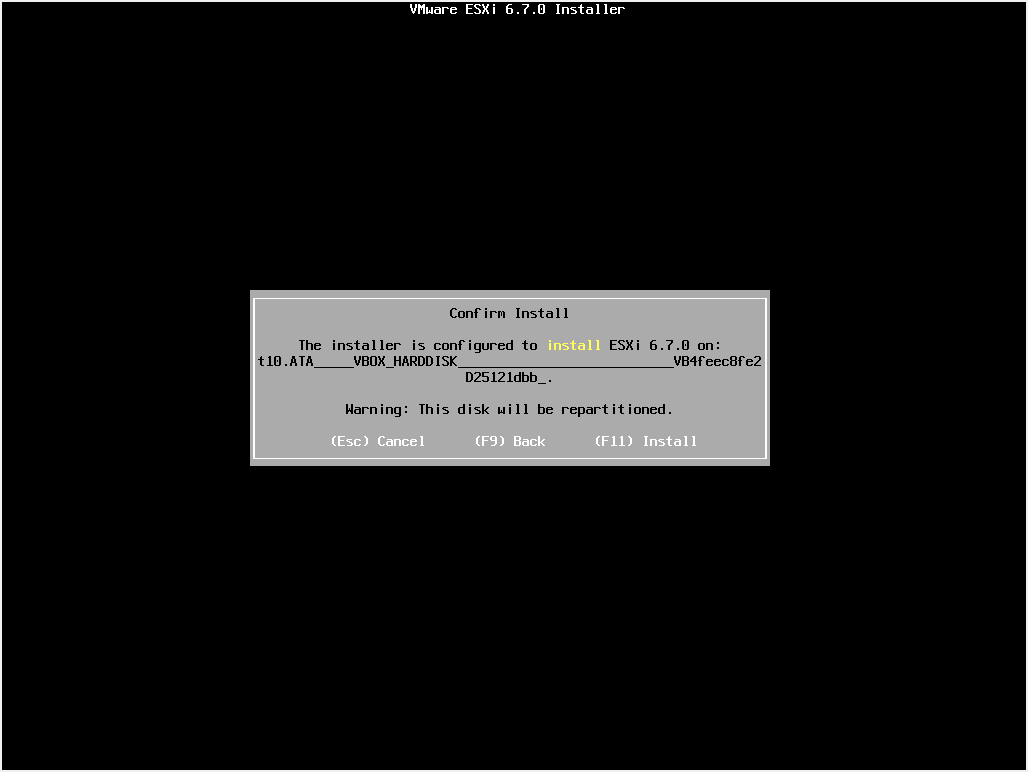
\includegraphics[width=\linewidth]{Trabajo/RecursosEducativos/RE01_VMwareESXi/RE_VMwareInstalacion11.png}
	\vspace{-0.2cm}
	\caption{Sitio Web WMWare \url{www.vmware.com}.\footnotemark[2]{} }
	\label{fig:VMwareInstalacion11}
\end{figure}


\begin{figure}[!hbtp]
	\centering
	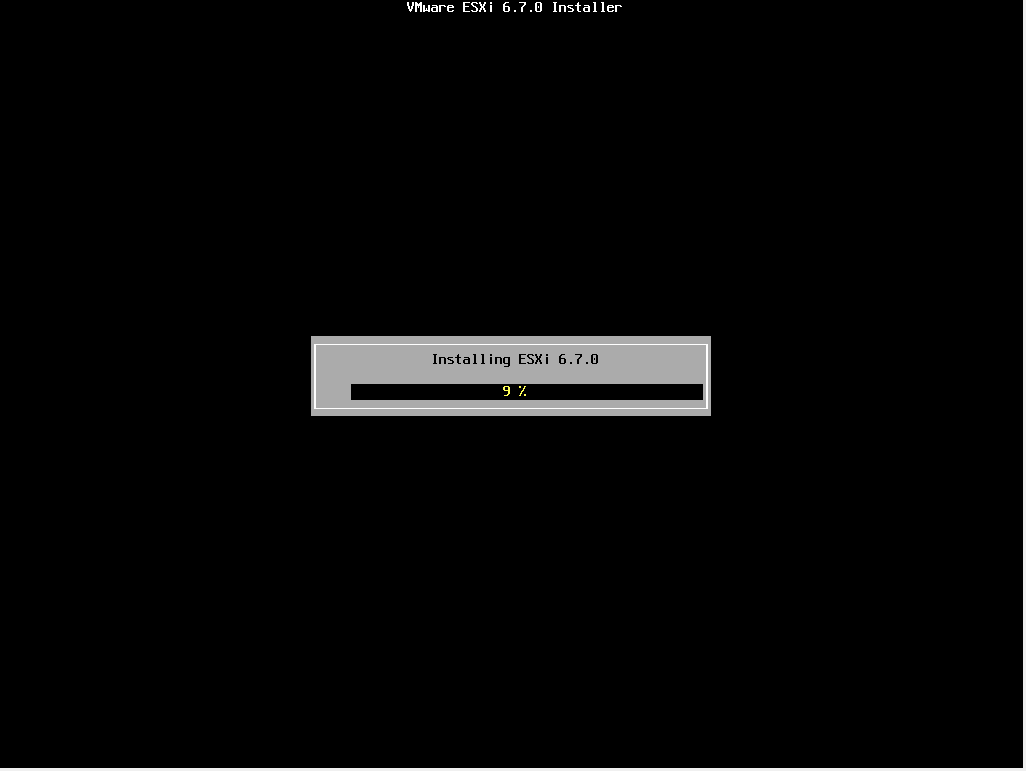
\includegraphics[width=\linewidth]{Trabajo/RecursosEducativos/RE01_VMwareESXi/RE_VMwareInstalacion12.png}
	\vspace{-0.2cm}
	\caption{Sitio Web WMWare \url{www.vmware.com}.\footnotemark[2]{} }
	\label{fig:VMwareInstalacion12}
\end{figure}


\begin{figure}[!hbtp]
	\centering
	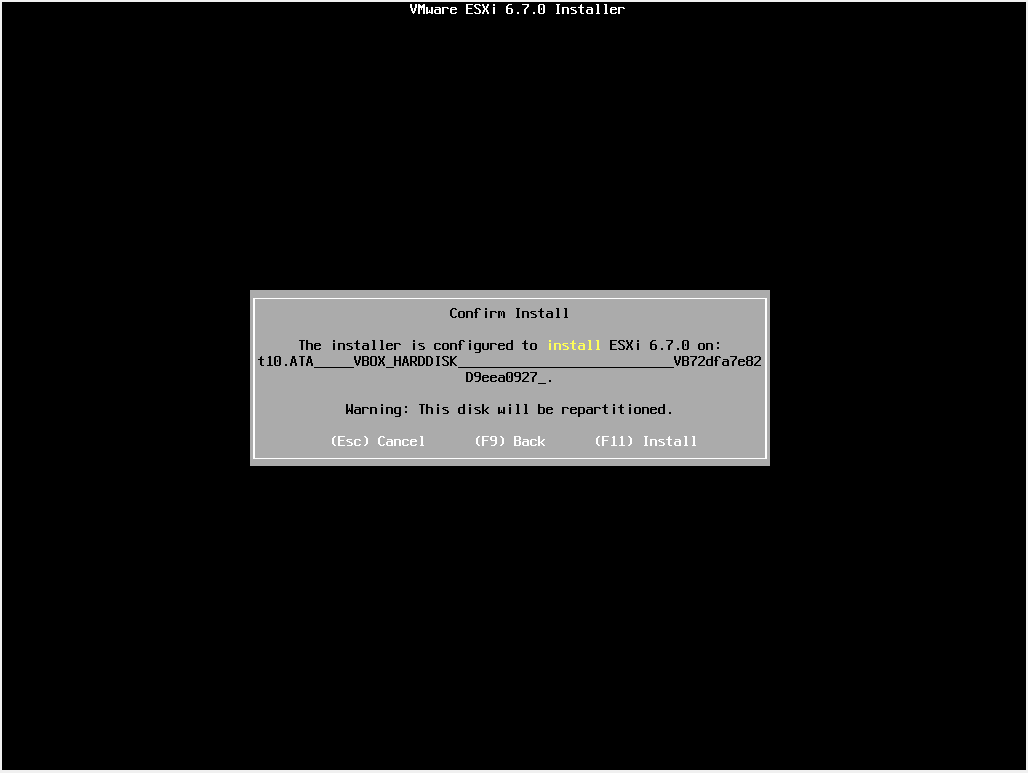
\includegraphics[width=\linewidth]{Trabajo/RecursosEducativos/RE01_VMwareESXi/RE_VMwareInstalacion13.png}
	\vspace{-0.2cm}
	\caption{Sitio Web WMWare \url{www.vmware.com}.\footnotemark[2]{} }
	\label{fig:VMwareInstalacion13}
\end{figure}


\begin{figure}[!hbtp]
	\centering
	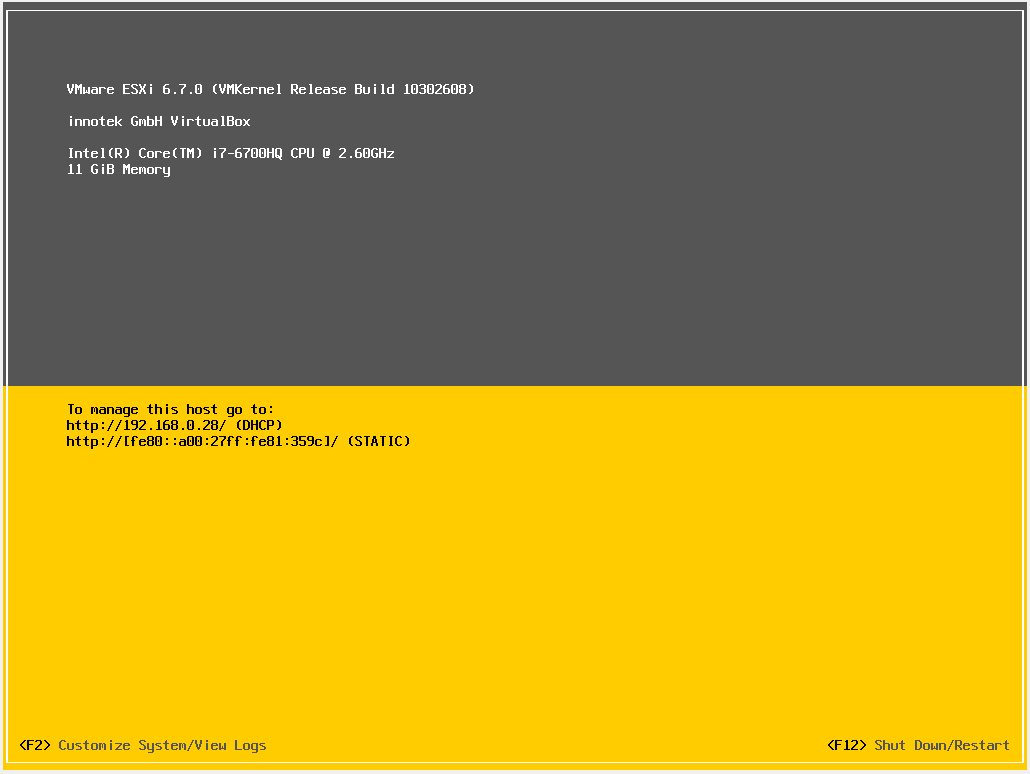
\includegraphics[width=\linewidth]{Trabajo/RecursosEducativos/RE01_VMwareESXi/RE_VMwareInstalacion14.png}
	\vspace{-0.2cm}
	\caption{Sitio Web WMWare \url{www.vmware.com}.\footnotemark[2]{} }
	\label{fig:VMwareInstalacion14}
\end{figure}


\begin{figure}[!hbtp]
	\centering
	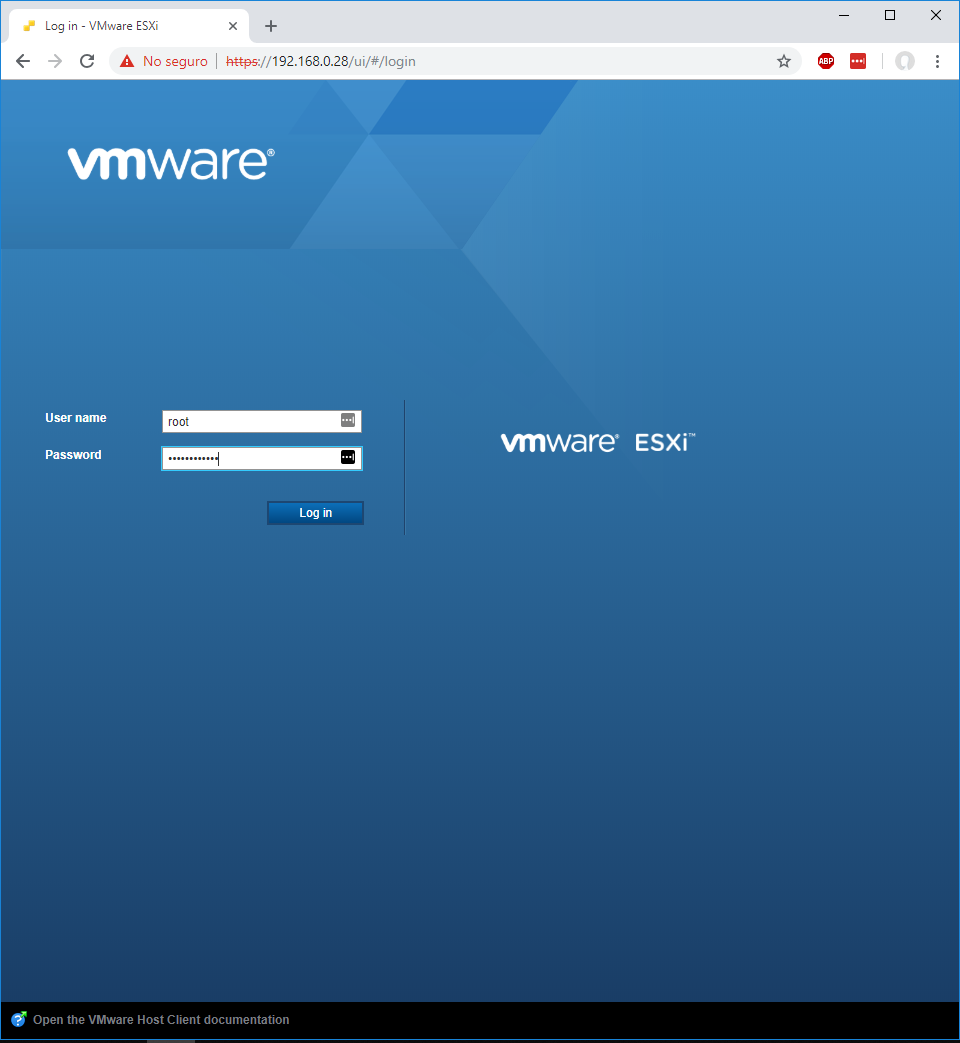
\includegraphics[width=\linewidth]{Trabajo/RecursosEducativos/RE01_VMwareESXi/RE_VMwareInstalacion15.png}
	\vspace{-0.2cm}
	\caption{Sitio Web WMWare \url{www.vmware.com}.\footnotemark[2]{} }
	\label{fig:VMwareInstalacion15}
\end{figure}

\begin{figure}[!hbtp]
	\centering
	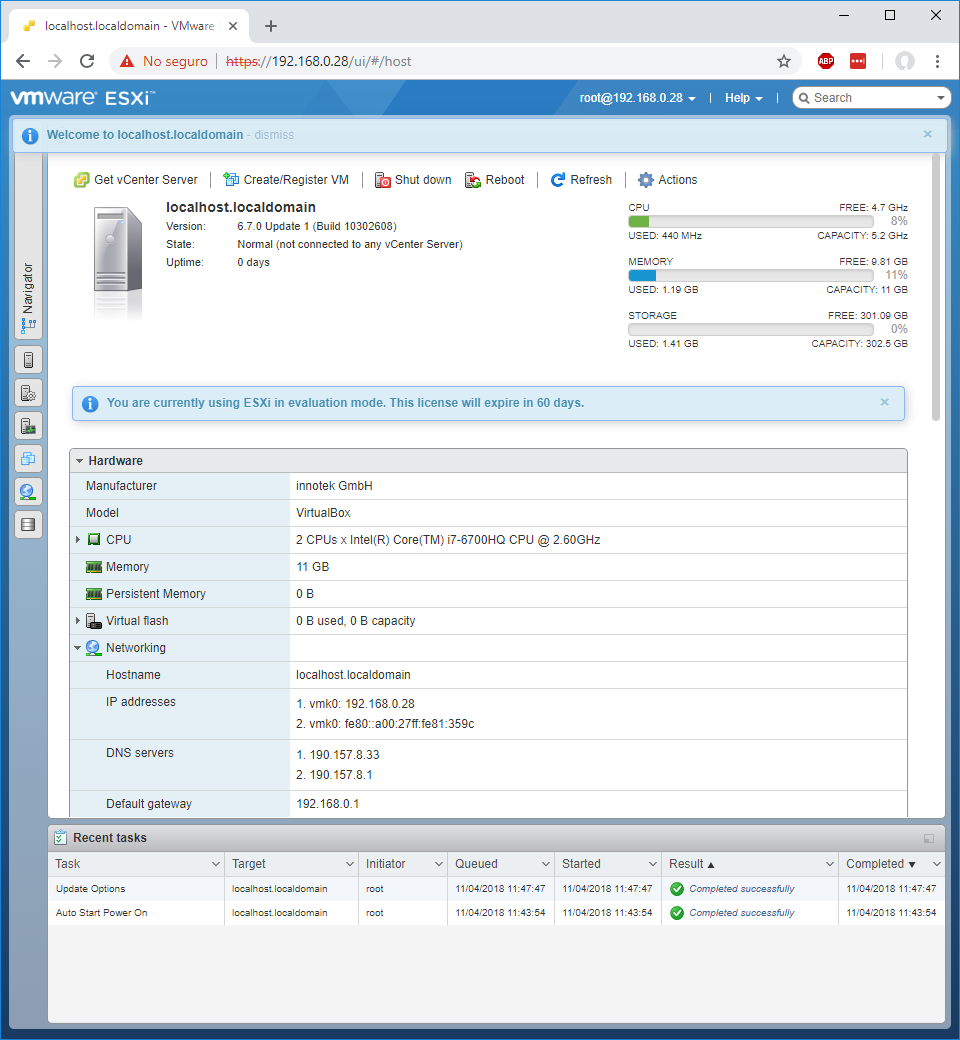
\includegraphics[width=\linewidth]{Trabajo/RecursosEducativos/RE01_VMwareESXi/RE_VMwareInstalacion16.png}
	\vspace{-0.2cm}
	\caption{Sitio Web WMWare \url{www.vmware.com}.\footnotemark[2]{} }
	\label{fig:VMwareInstalacion16}
\end{figure}

\subsubsection{Instalación de VCenter}

Para la instalación de una versión de prueba de VCenter es necesario tener la ISO del appliance, la cual se puede descargar de la página oficial de VMWare como se muestra en la siguiente imagen.






\newpage

\subsection{Recurso Educativo para la herramienta Docker}
%%%%%%%%%%%%%%%%%%%%%%%%%%%%%%%%%
%% PROPOSITO GENERAL
%%%%%%%%%%%%%%%%%%%%%%%%%%%%%%%%%
\subsubsection{Propósito}

Docker es una plataforma abierta que tiene como propósito permitir el desarrollo, envío y ejecución de aplicaciones, permitiendo separar el software de la infraestructura para que se pueda entregar software rápidamente \parencite{Docker2018}.

Es importante aclarar que Docker tiene tanto una versión empresarial llamada Docker EE (Enterprise Edition) y una versión comunitaria llamada Docker CE (Community Edition) ver figura \ref{fig:DockerVersiones}. Para el presente trabajo se utiliza la versión comunitaria.

\begin{figure}[!hbtp]
	\centering
	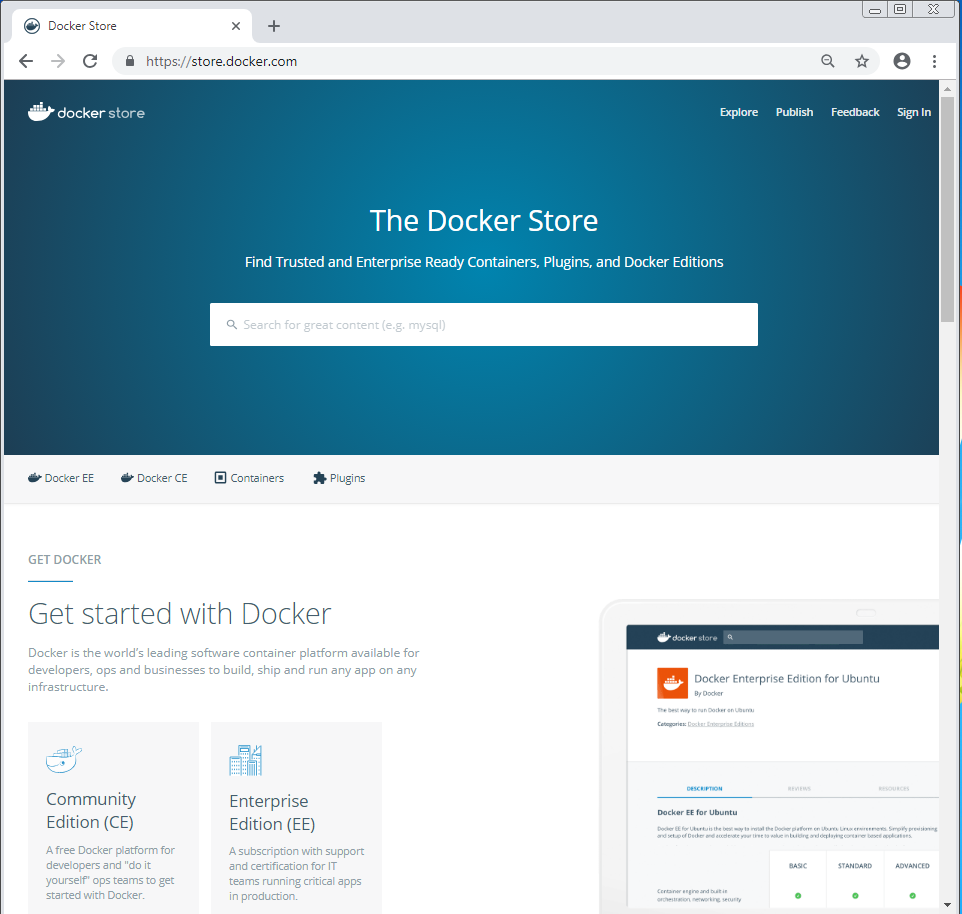
\includegraphics[width=\linewidth]{Trabajo/RecursosEducativos/RE05_Docker/REDocker_versiones.png}
	\vspace{-0.2cm}
	\caption{Sitio web The Docker Store \url{https://store.docker.com/}.}
	\label{fig:DockerVersiones}
\end{figure}

%%%%%%%%%%%%%%%%%%%%%%%%%%%%%%%%%
%% ASPECTOS TEC GENERALES
%%%%%%%%%%%%%%%%%%%%%%%%%%%%%%%%%

\subsection{Aspectos técnicos generales}

Según \textcite{Docker2018} Docker ofrece la capacidad de empaquetar y ejecutar aplicaciones en un entorno aislado y holgado llamado contenedor, el aislamiento y la seguridad permite ejecutar muchos contenedores simultáneamente en un mismo host. Adicional \textcite{Docker2018} indica que los contenedores son livianos porque no necesitan la carga de un hipervisor, debido a que se ejecutan directamente en el nucleo del equipo host, incluso dentro de máquinas virtuales que se encuentren en un host.

Docker proporciona una plataforma y herramientas para la administración del ciclo de vida de sus contenedores:
\begin{itemize}
    \item Desarrolle sus aplicaciones y componentes de soporte utilizando Docker.
    \item El contenedor creado se convierte en la unidad para distribuir y probar la aplicación.
    \item Cuanto todo este listo y funcional, puede desplegar la aplicación o el servicio en producción de la misma forma sin importar que el entorno de producción sea un datacenter, una nube pública o privada.
\end{itemize}

Según \textcite{Docker2018} cuando se utiliza Docker se crean y se utilizan contenedores, imágenes, volúmenes, redes, complementos, entre otras cosas. En esta sección se procede a describir que es una imagen y un contenedor.

\textbf{Imágenes}
Una imagen es una plantilla de solo lectura con instrucciones para crear un contenedor Docker. A menudo, una imagen se basa en otra imagen, con alguna personalización adicional. Por ejemplo, puede crear una imagen basada en la imagen de ubuntu, pero instala el servidor web Apache y su aplicación, así como los detalles de configuración necesarios para hacer que su aplicación se ejecute. \parencite{Docker2018}.

\textbf{Contenedores}
Un contenedor es una instancia ejecutable de una imagen. Puede crear, iniciar, detener, mover o eliminar un contenedor utilizando la API o la CLI de Docker. Puede conectar un contenedor a una o más redes, adjuntarle almacenamiento o incluso crear una nueva imagen según su estado actual. Un contenedor se define por su imagen, así como por las opciones de configuración que le proporciona al crearlo o iniciarlo. Cuando se elimina un contenedor, desaparecen todos los cambios en su estado que no se almacenan en el almacenamiento persistente. \parencite{Docker2018}


%%%%%%%%%%%%%%%%%%%%%%%%%%%%%%%%%
%% ARQUITECTURA
%%%%%%%%%%%%%%%%%%%%%%%%%%%%%%%%%
\subsubsection{Arquitectura}

Como se puede observar en la figura \ref{fig:DockerArquitectura} y según lo establece \textcite{Docker2018} Docker utiliza una arquitectura de cliente servidor. En la cual el cliente Docker habla con el Demonio de Docker encargado de construir, ejecutar y distribuir los contenedores Docker. El cliente y el demonio pueden estar en ejecución en el mismo host o en host remotos, debido a que se pueden comunicar a través de API Rest, Sockets Unix o interfaces de red.

\begin{figure}[!hbtp]
	\centering
	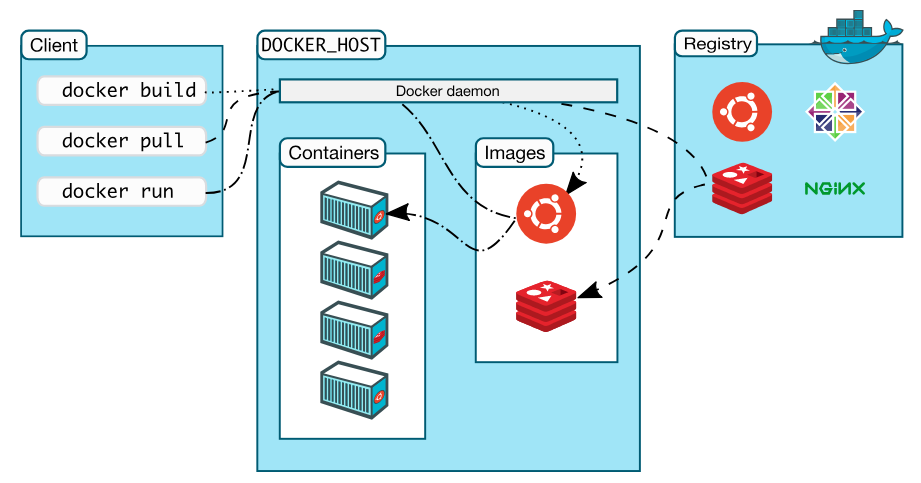
\includegraphics[width=\linewidth]{Trabajo/RecursosEducativos/RE05_Docker/REDocker_Arquitectura.png}
	\vspace{-0.2cm}
	\caption{Sitio web Docker Docs \url{https://docs.docker.com/engine/docker-overview/}.}
	\label{fig:DockerArquitectura}
\end{figure}

En la figura \ref{fig:DockerArquitectura} se encuentran los siguientes componentes:
\textbf{The Docker Daemon (El demonio de docker)}
El demonio de Docker (dockerd) escucha las solicitudes de la API de Docker y administra los objetos de Docker, como imágenes, contenedores, redes y volúmenes. Un demonio también puede comunicarse con otros demonios para administrar los servicios de Docker. \parencite{Docker2018}

\textbf{The Docker Client (El cliente de Docker)}
El cliente Docker (docker) es la forma principal en que muchos usuarios de Docker interactúan con Docker. Cuando utiliza comandos como la ejecución de la ventana acoplable, el cliente envía estos comandos a dockerd, que los ejecuta. El comando docker utiliza la API de Docker. El cliente Docker puede comunicarse con más de un demonio.\parencite{Docker2018}

\textbf{Docker Registries (Registros de Docker)}
Un registro de Docker es donde se almacenan las imágenes de Docker. Docker Hub es un registro público que cualquiera puede usar. Docker está configurado para buscar imágenes en Docker Hub de forma predeterminada. Es posible tener un registro de imágenes privado. \parencite{Docker2018}

%%%%%%%%%%%%%%%%%%%%%%%%%%%%%%%%%
%% INSTALACION LINUX
%%%%%%%%%%%%%%%%%%%%%%%%%%%%%%%%%
\subsection{Instalación en Linux}
Para la instalación de Docker CE en los sistemas operativos GNU/Linux se tienen diferentes métodos como la instalación de los repositorios, descargar los ejecutables para la distribución específica o la ejecución de un script que contiene los pasos de instalación básica, la ejecución del script se realiza con los siguientes comandos, y su salida se puede observar en la figura \ref{fig:InstalacionDockerLinux1}

\begin{figure}[!hbtp]
	\centering
	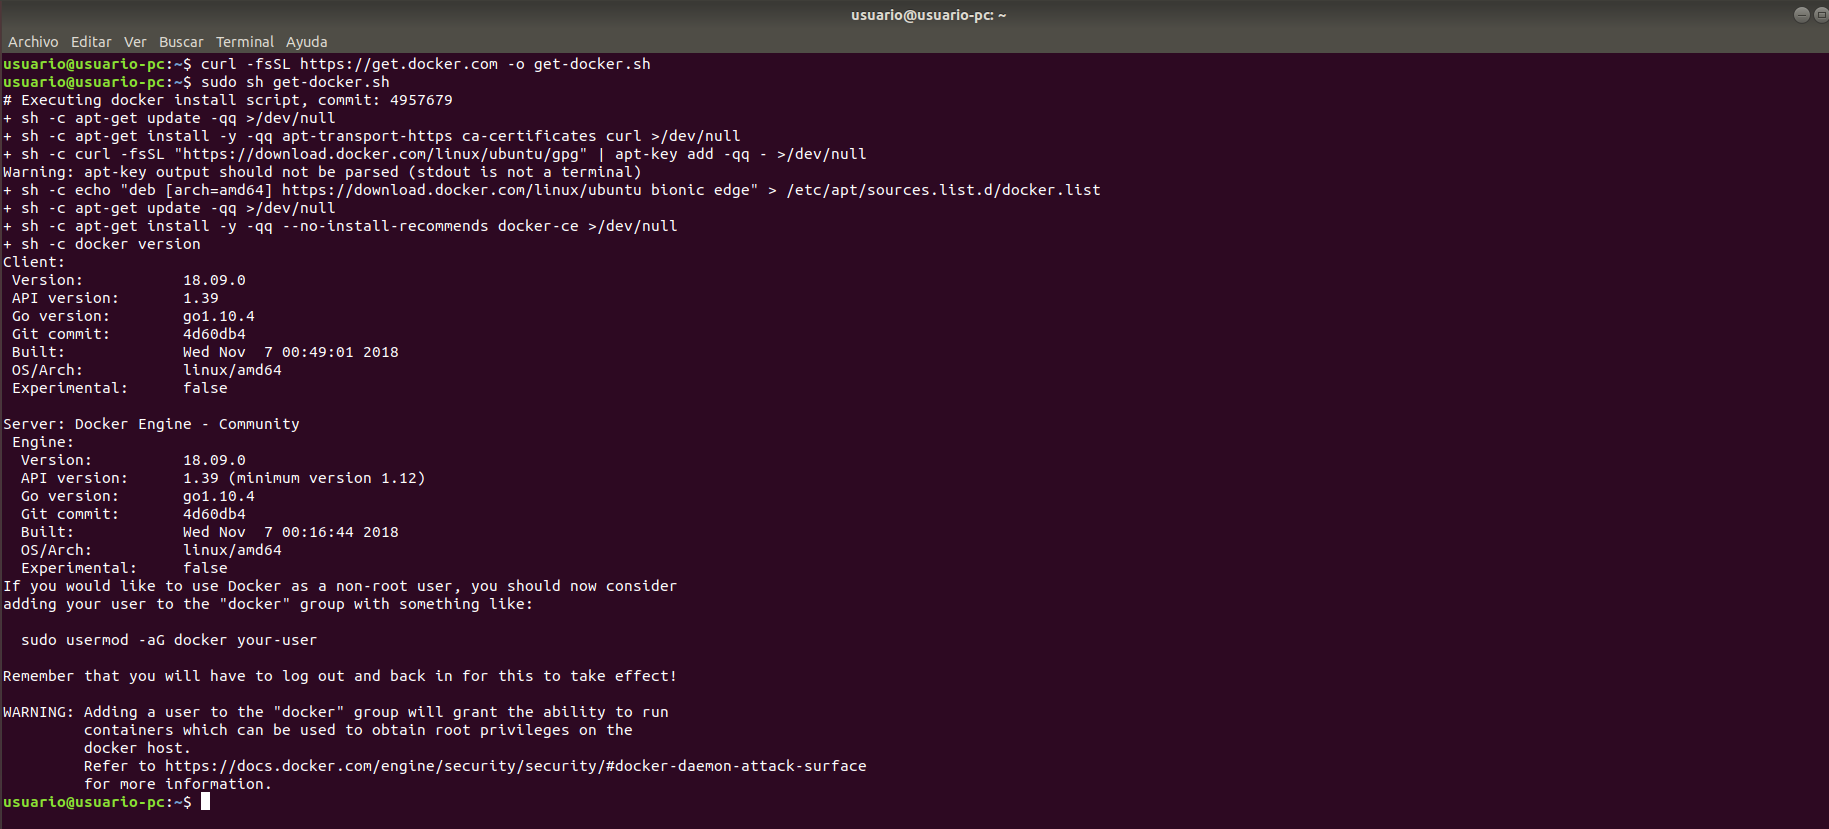
\includegraphics[width=\linewidth]{Trabajo/RecursosEducativos/RE05_Docker/Instalacion_Linux/REDocker_Instalacion_Linux.png}
	\vspace{-0.2cm}
	\caption{Salida del script de instalación Docker }
	\label{fig:InstalacionDockerLinux1}
\end{figure}

Al terminar la instalación de Docker CE se puede verificar la versión básica de Docker con el comando \begin{commandshell}{docker version}\end{commandshell}
en la figura \ref{fig:InstalacionDockerLinux2} se puede ver la salida del comando.

\begin{figure}[!hbtp]
	\centering
	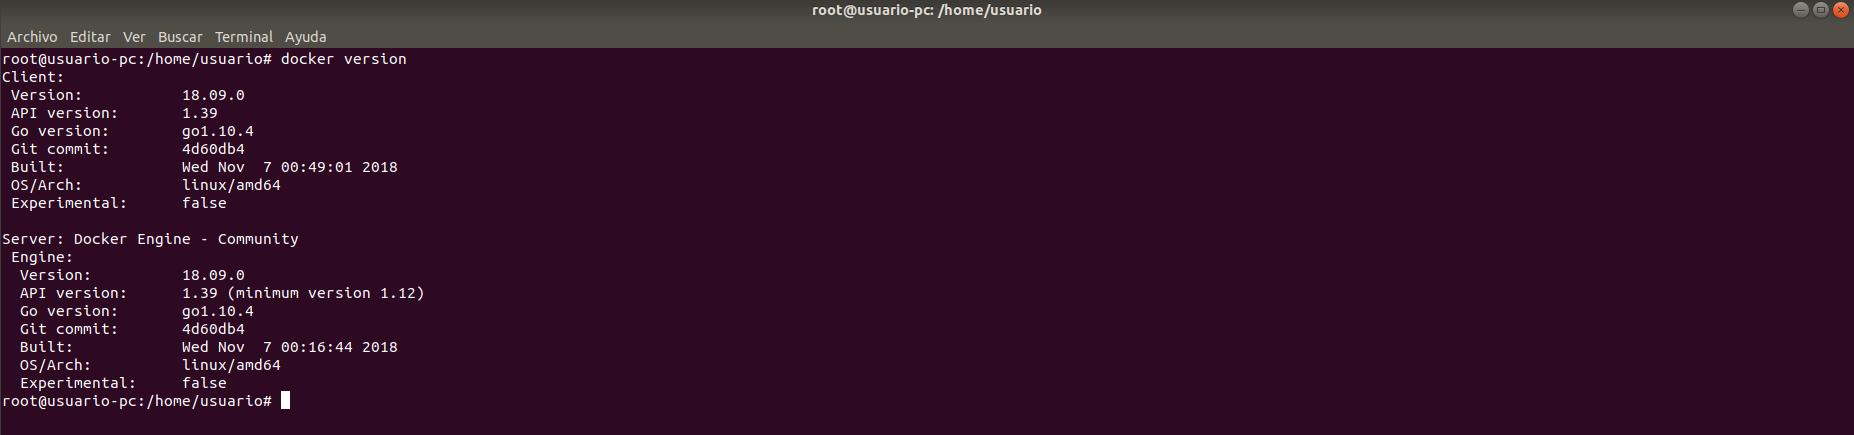
\includegraphics[width=\linewidth]{Trabajo/RecursosEducativos/RE05_Docker/Instalacion_Linux/REDocker_Instalacion_Linux2.png}
	\vspace{-0.2cm}
	\caption{Salida del comando docker version }
	\label{fig:InstalacionDockerLinux2}
\end{figure}
%%%%%%%%%%%%%%%%%%%%%%%%%%%%%%%%%
%% INSTALACION Windows
%%%%%%%%%%%%%%%%%%%%%%%%%%%%%%%%%
\subsection{Instalación Microsoft Windows}
Para poder realizar la instalación de Docker en microsoft windows de una forma nativa, sólo funcionará con las versiones Microsoft Windows 10 Professional y Microsoft Windows 10 Enterprise, en las figuras \ref{fig:InstalacionDockerWin1},\ref{fig:InstalacionDockerWin2},\ref{fig:InstalacionDockerWin3},\ref{fig:InstalacionDockerWin4} se muestra la interacción con el asistente de instalación de Docker.

\begin{figure}[!hbtp]
	\centering
	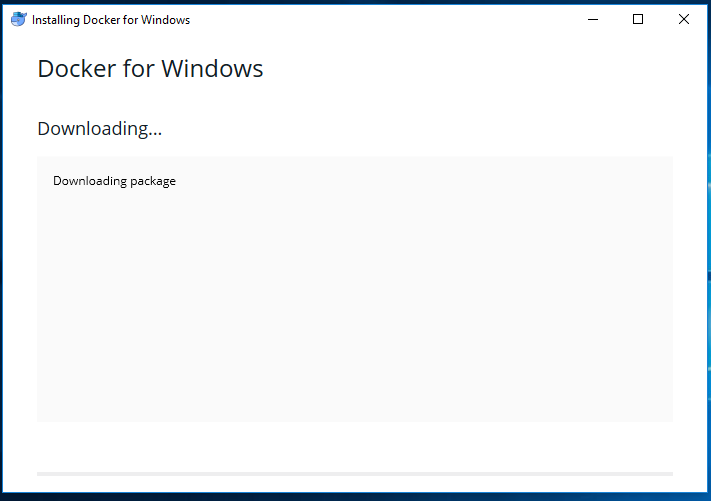
\includegraphics[width=\linewidth]{Trabajo/RecursosEducativos/RE05_Docker/Instalacion_Windows/REDocker_Instalacion_Windows01.png}
	\vspace{-0.2cm}
	\caption{Asistente instalación Docker: Descarga paquetes necesarios}
	\label{fig:InstalacionDockerWin1}
\end{figure}

\begin{figure}[!hbtp]
	\centering
	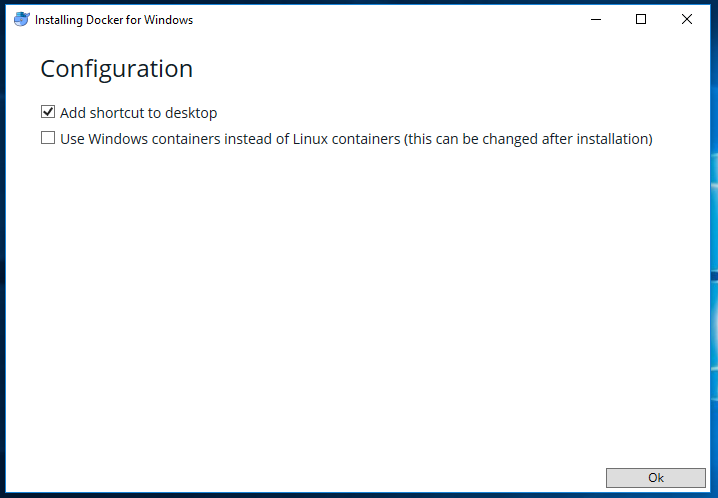
\includegraphics[width=\linewidth]{Trabajo/RecursosEducativos/RE05_Docker/Instalacion_Windows/REDocker_Instalacion_Windows02.png}
	\vspace{-0.2cm}
	\caption{Asistente instalación Docker: Configuración básica}
	\label{fig:InstalacionDockerWin2}
\end{figure}

\begin{figure}[!hbtp]
	\centering
	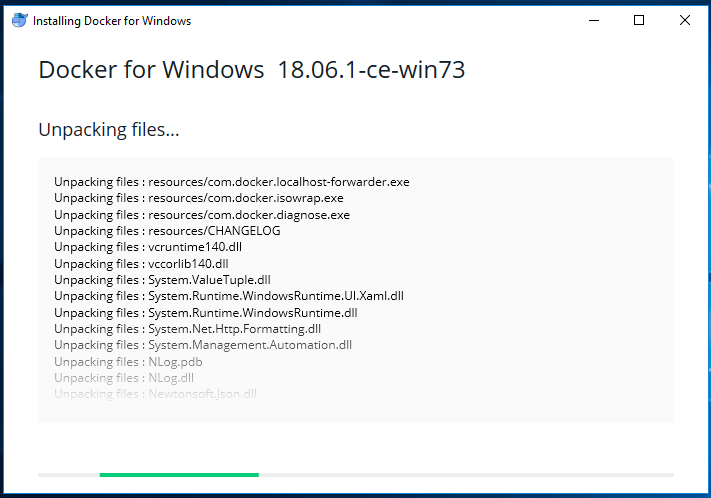
\includegraphics[width=\linewidth]{Trabajo/RecursosEducativos/RE05_Docker/Instalacion_Windows/REDocker_Instalacion_Windows03.png}
	\vspace{-0.2cm}
	\caption{Asistente instalación Docker: Descompresión de paquetes}
	\label{fig:InstalacionDockerWin3}
\end{figure}

\begin{figure}[!hbtp]
	\centering
	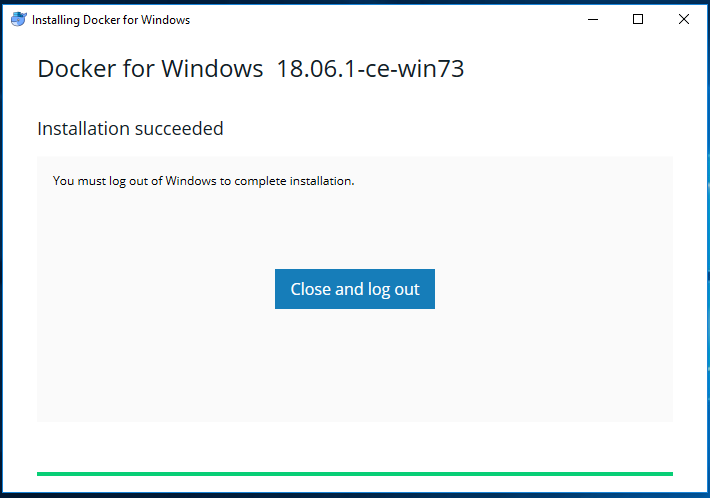
\includegraphics[width=\linewidth]{Trabajo/RecursosEducativos/RE05_Docker/Instalacion_Windows/REDocker_Instalacion_Windows04.png}
	\vspace{-0.2cm}
	\caption{Asistente instalación Docker: Finalización del asistente}
	\label{fig:InstalacionDockerWin4}
\end{figure}

En caso de que se tengan versiones de Microsoft Windows anteriores se puede utilizar Docker Tool Box, herramienta que permite a través de una máquina virtual la gestión de contenedores Docker. Para conocer el proceso de instalación se puede ver el Anexo 2.

%%%%%%%%%%%%%%%%%%%%%%%%%%%%%%%%%
%% GESTION BÁSICA 
%%%%%%%%%%%%%%%%%%%%%%%%%%%%%%%%%
\subsection{Gestión básica de Docker}

Es esta sección s van a mostrar algunos comandos básicos para la gestión básica de imagenes, contenedores, entre otros.

\textbf{Consulta de información Docker}

Para ver la información general de la instalación de docker sus contenedores, imagenes y demás información relevante se utiliza el comando \begin{commandshell}docker info\end{commandshell} 
en la figura \ref{fig:DockerGestion1} se puede ver la salida del comando.

\begin{figure}[!hbtp]
	\centering
	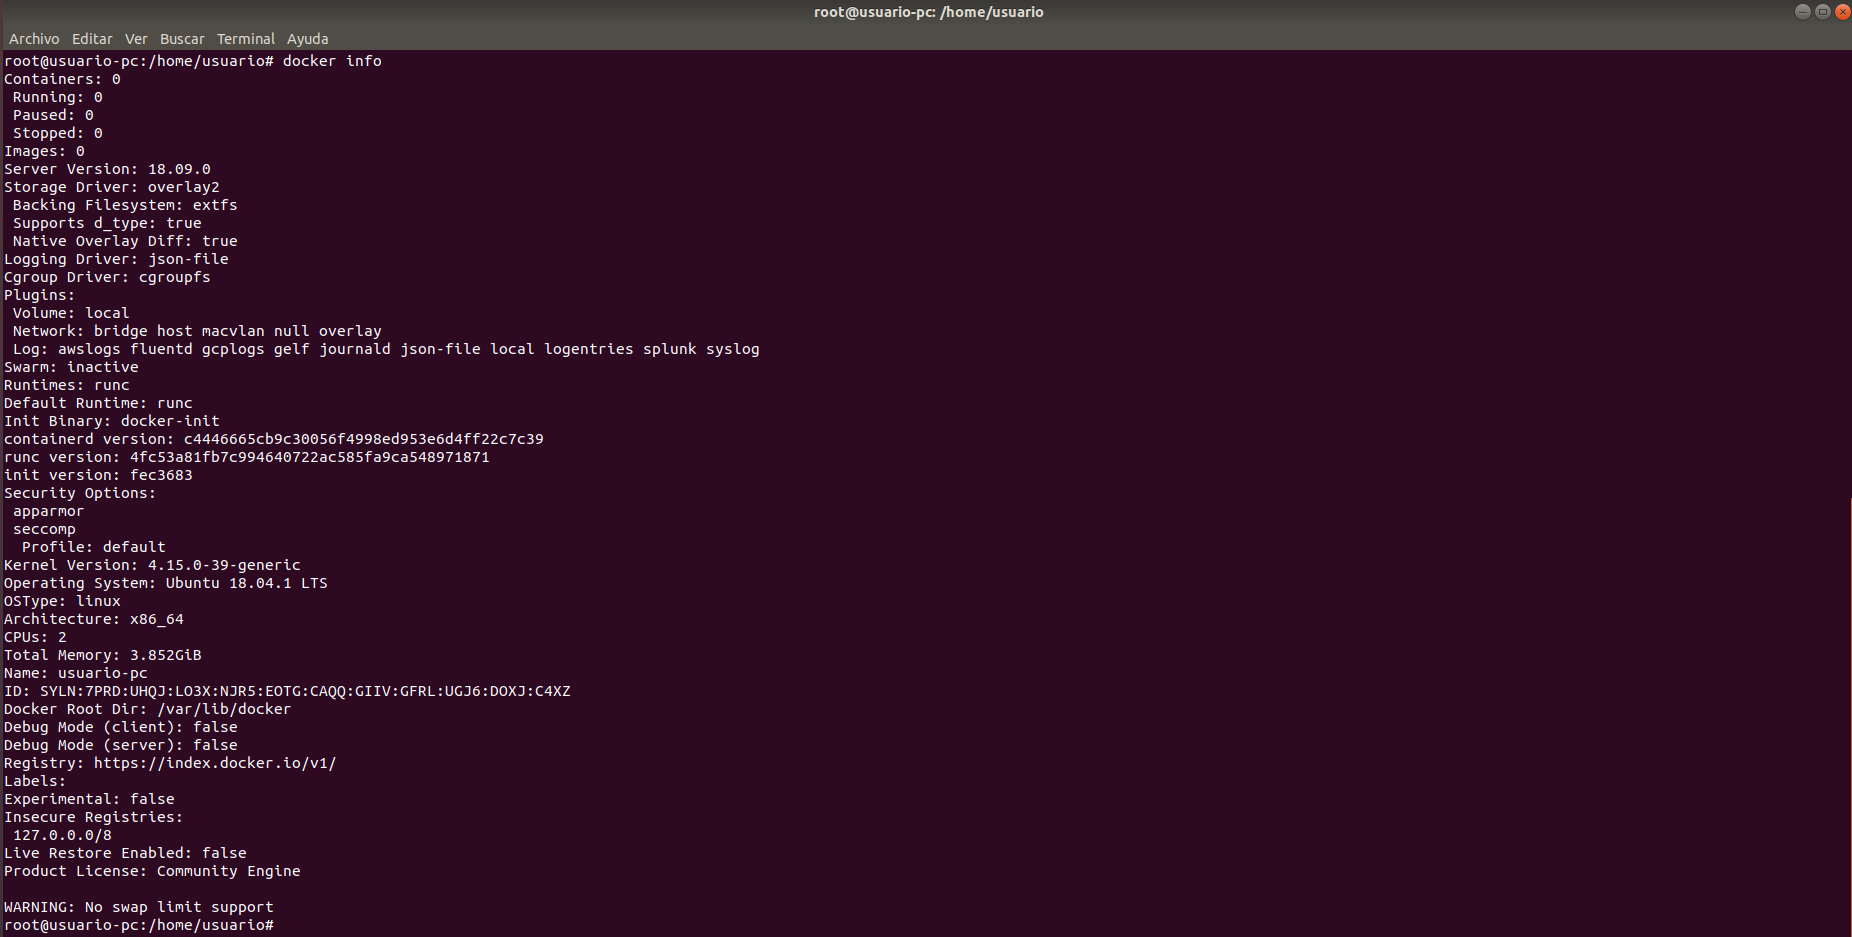
\includegraphics[width=\linewidth]{Trabajo/RecursosEducativos/RE05_Docker/Gestion_basica/REDocker_Gestion1.png}
	\vspace{-0.2cm}
	\caption{Salida del comando docker info}
	\label{fig:DockerGestion1}
\end{figure}
%%%%%%%%%%%%%%%%%%%%%%%%%%%%%%%%%
%% GESTIÓN DE IMAGENES
%%%%%%%%%%%%%%%%%%%%%%%%%%%%%%%%%
\textbf{Consulta de imágenes existentes en el host}

Para listar las imágenes descargadas en el host que actualmente ejecuta docker se utiliza el siguiente comando  \begin{commandshell}docker images\end{commandshell}

En la imagen \ref{fig:DockerGestion2} se puede observar la salida del comando destacando la siguiente información:
\begin{itemize}
    \item REPOSITORY: Nombre del repositorio donde proviene la imagen.
    \item TAG: Es utilizado para nombrar las versiones de una imagen, es decir, a medida que se se introducen cambios a una imagen se puede asociar con un nuevo TAG, facilitando el control de versiones de las imagenes.
    \item IMAGE ID: Número de identificación único para cada imagen.
    \item CREATE: Indica el momento en el que fue creada la imagen.
    \item SIZE: Indica el tamaño en disco de la imagen.
\end{itemize}

\begin{figure}[!hbtp]
	\centering
	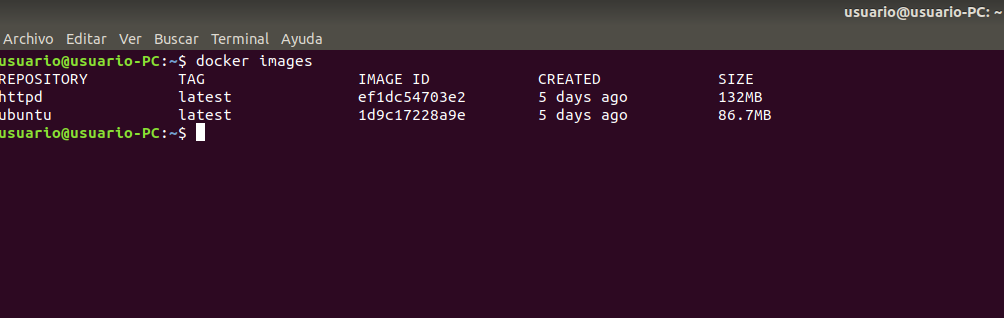
\includegraphics[width=\linewidth]{Trabajo/RecursosEducativos/RE05_Docker/Gestion_basica/REDocker_Gestion2.png}
	\vspace{-0.2cm}
	\caption{Salida del comando docker images}
	\label{fig:DockerGestion2}
\end{figure}
%%%%%%%%%%%%%%%%%%%%%%%%%%%%%%%%%
%% BUSQUEDA EN DOCKER HUB
%%%%%%%%%%%%%%%%%%%%%%%%%%%%%%%%%
\textbf{Búsqueda de imágenes en repositorio}

Docker apoyado en su comunidad a través de Docker Hub ver figura \ref{fig:DockerGestion4} ofrece un servicio para buscar y compartir imágenes de contenedores. Para poder buscar las imagenes disponibles es necesaria la creación de una cuenta.

\begin{figure}[!hbtp]
	\centering
	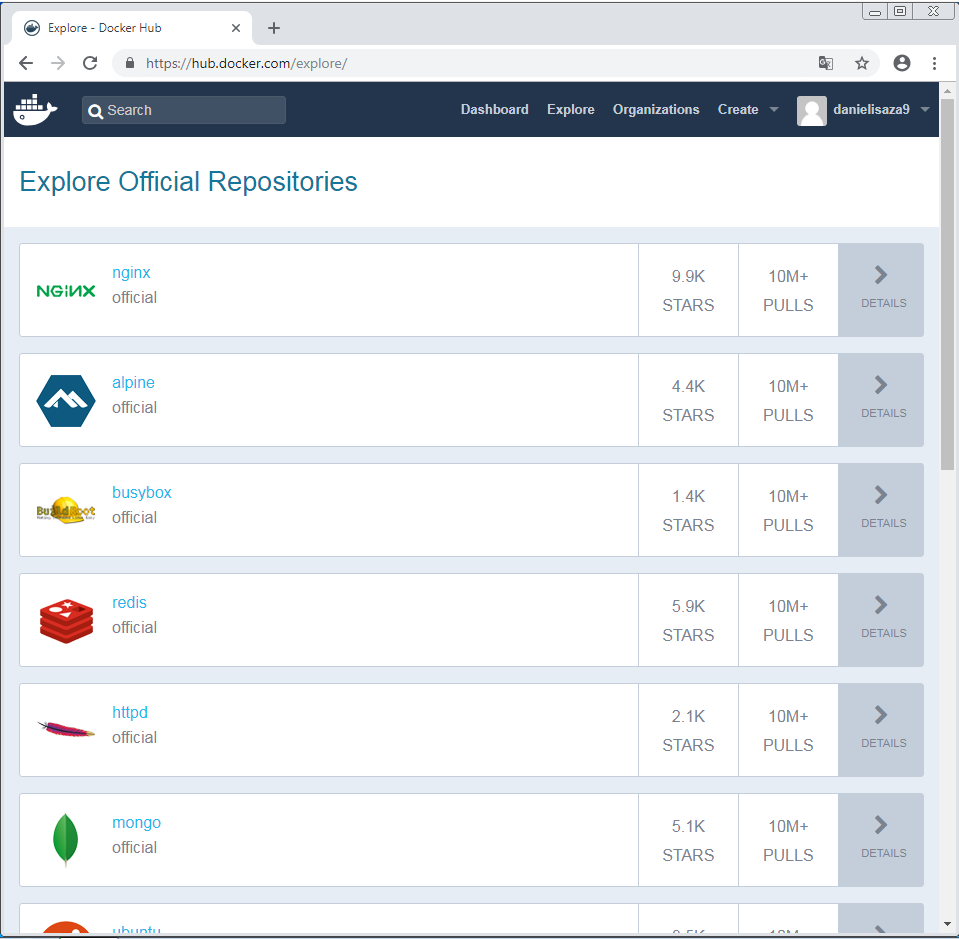
\includegraphics[width=\linewidth]{Trabajo/RecursosEducativos/RE05_Docker/Gestion_basica/REDocker_Gestion4.png}
	\vspace{-0.2cm}
	\caption{Sitio web Docker Hub \url{https://hub.docker.com/explore/}.}
	\label{fig:DockerGestion4}
\end{figure}

Para buscar una imagen alojada en Docker Hub para su posible descarga se utiliza el comando 
\begin{commandshell}docker search nombreImagen\end{commandshell}

En la figura \ref{fig:DockerGestion3} se ve la salida del comando para la búsqueda de imágenes que tengan la palabra ubuntu.

\begin{figure}[!hbtp]
	\centering
	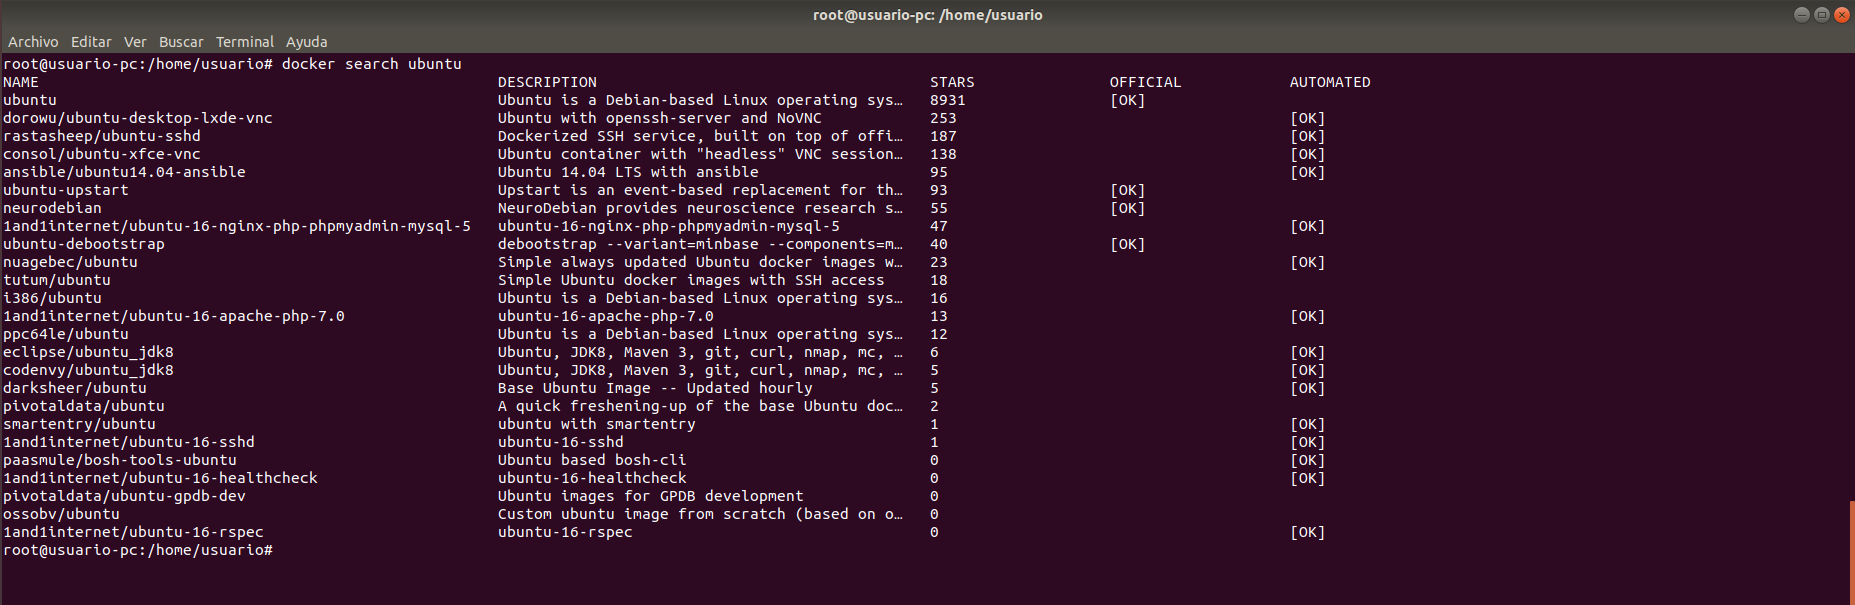
\includegraphics[width=\linewidth]{Trabajo/RecursosEducativos/RE05_Docker/Gestion_basica/REDocker_Gestion3.png}
	\vspace{-0.2cm}
	\caption{Salida comando docker search ubuntu}
	\label{fig:DockerGestion3}
\end{figure}

%%%%%%%%%%%%%%%%%%%%%%%%%%%%%%%%%
%% DESCARGA IMAGENES
%%%%%%%%%%%%%%%%%%%%%%%%%%%%%%%%%
\textbf{Descarga de una imagen}
Una vez que se identifica el nombre de la imagen que se desea descargar de Docker Hub, por ejemplo la imagen hello-world que se envia como argumento del comando pull de la siguiente forma:
\begin{commandshell} docker pull hello-world \end{commandshell}

La salida del comando se puede observar en la figura \ref{fig:DockerGestion5} donde se muestra la descarga exitosa de la imagen y la verificación de que la misma exista. 

\begin{figure}[!hbtp]
	\centering
	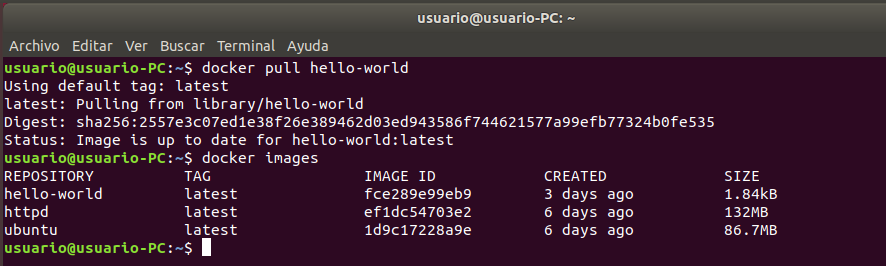
\includegraphics[width=\linewidth]{Trabajo/RecursosEducativos/RE05_Docker/Gestion_basica/REDocker_Gestion5.png}
	\vspace{-0.2cm}
	\caption{Salida comando docker search ubuntu}
	\label{fig:DockerGestion5}
\end{figure}

También es posible agregar el TAG al comando de descarga de imágenes, permitiendo establecer la versión especifica que se desea obtener, como se muestra en el siguiente comando:

\begin{commandshell} docker pull hello-world:latest \end{commandshell}

%%%%%%%%%%%%%%%%%%%%%%%%%%%%%%%%%
%% CREACION CONTENEDORES
%%%%%%%%%%%%%%%%%%%%%%%%%%%%%%%%%
\textbf{Creación de un contenedor}
Para poder crear un nuevo contenedor es necesario conocer el nombre de la imagen que se desea utilizar, no es necesario que la imagen se encuentre disponible localmente, en dicho caso docker procede con la búsqueda y descarga desde Docker Hub.  

Un ejemplo de imagen clásico es la de hello-world que sigue la tradición del primer programa que se crea cuando se aprende a programar, el comando para crear el contenedor es el siguiente

\begin{commandshell} docker run hello-world \end{commandshell}

En la figura \ref{fig:DockerGestion6} se puede observar la salida del comando y se puede identificar que al ejecutar un contenedor utilizando la imagen hello-world se verifica el correcto funcionamiento de docker.

\begin{figure}[!hbtp]
	\centering
	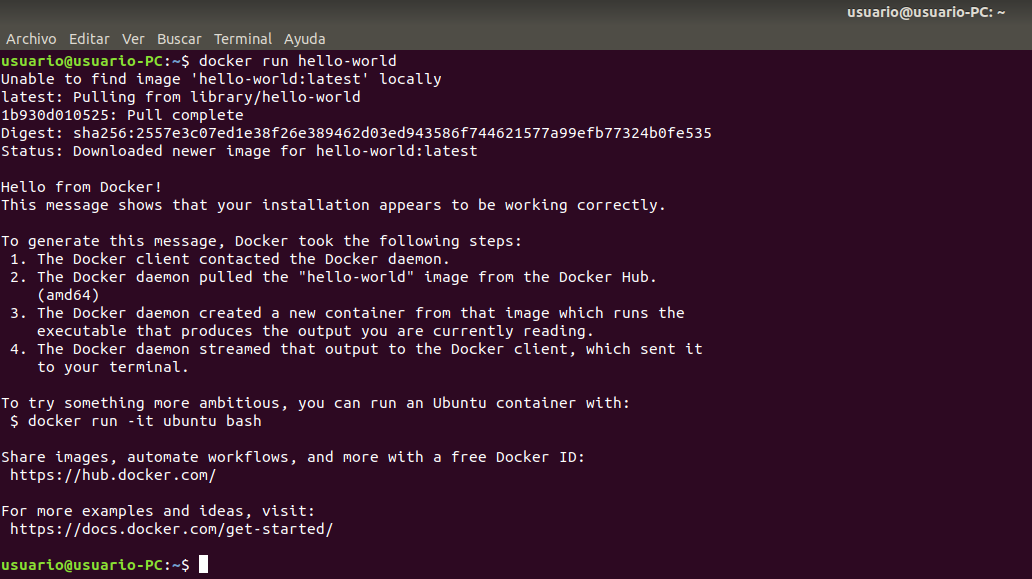
\includegraphics[width=\linewidth]{Trabajo/RecursosEducativos/RE05_Docker/Gestion_basica/REDocker_Gestion6.png}
	\vspace{-0.2cm}
	\caption{Salida comando docker run hello-world}
	\label{fig:DockerGestion6}
\end{figure}

Para listar los contenedores que se han creado en el host ya sea que se encuentren en ejecución se utiliza el siguiente comando
\begin{commandshell} docker ps \end{commandshell}

En caso de que se deseen ver todos los contenedores en ejecución y que ya se encuentran detenidos, se agrega la opción -a tal como se ve en el siguiente comando
\begin{commandshell} docker ps -a \end{commandshell}

La salida de los comandos mostrados anteriormente se ve reflejada en la figura \ref{fig:DockerGestion7}, la cual contiene la siguiente información: 
\begin{itemize}
    \item CONTAINER ID: Número único de identificación para el contenedor en el host actual.
    \item IMAGE: Nombre de la imagen y etiqueta utilizados para la creación del contenedor.
    \item COMMAND: Hace referencia al comando citado al momento de ejecutar el contenedor.
    \item CREATED: Indica el momento de creación del contenedor.
    \item STATUS: Muestra el estado del contenedor, en caso de que se encuentre detenido indica el tiempo de terminación.
    \item PORTS: Indica el puerto TCP del host que se utiliza para escuchar un puerto específico del contenedor.
    \item NAMES: Hace referencia al nombre dado al contenedor ya sea de forma aleatoria o manual. 
\end{itemize}

\begin{figure}[!hbtp]
	\centering
	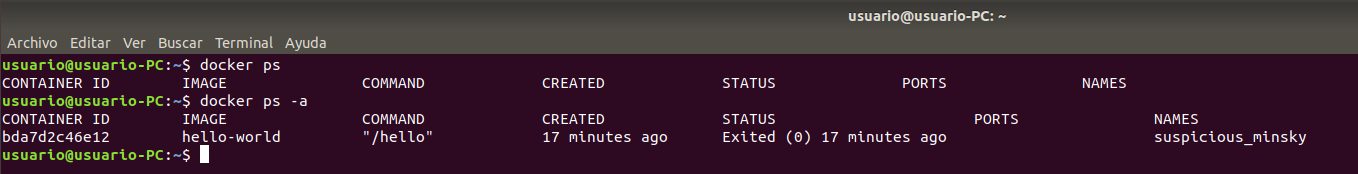
\includegraphics[width=\linewidth]{Trabajo/RecursosEducativos/RE05_Docker/Gestion_basica/REDocker_Gestion7.png}
	\vspace{-0.2cm}
	\caption{Salida comandos docker ps  docker ps -a}
	\label{fig:DockerGestion7}
\end{figure}
%%%%%%%%%%%%%%%%%%%%%%%%%%%%%%%%%
%% EJECUCION COMANDOS CONTENEDORES
%%%%%%%%%%%%%%%%%%%%%%%%%%%%%%%%%
\textbf{Ejecutar comandos en contenedores}
A través del comando \texttt{docker run} es posible crear contenedores y ejecutar comandos en los mismos. Por ejemplo, para ejecutar el comando ls -l en un contenedor creado con una imagen de ubuntu, se deben ejecutar los siguientes comandos:
\begin{commandshell}
docker pull ubuntu:latest
docker run ubuntu ls -l /
\end{commandshell}

El resultado de la ejecución del comando ls -l en ubuntu, se puede observar en la figura \ref{fig:DockerGestion8} donde se ven los directorios ubicados en raíz.

\begin{figure}[!hbtp]
	\centering
	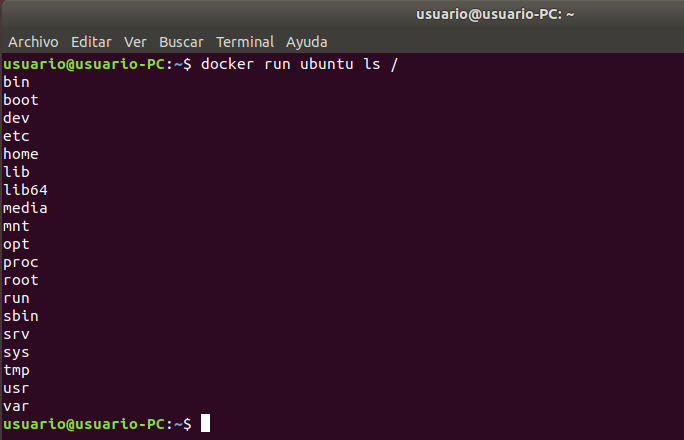
\includegraphics[width=\linewidth]{Trabajo/RecursosEducativos/RE05_Docker/Gestion_basica/REDocker_Gestion8.png}
	\vspace{-0.2cm}
	\caption{Salida comando docker run ubuntu ls -l /}
	\label{fig:DockerGestion8}
\end{figure}
%%%%%%%%%%%%%%%%%%%%%%%%%%%%%%%%%
%% EJECUCION COMANDOS CONTENEDORES
%%%%%%%%%%%%%%%%%%%%%%%%%%%%%%%%%
\textbf{Terminar interactiva}
En algunas ocasiones puede ser necesario gestionar direcctamente los contenedores a través de una terminal. Para lograr lo anterior, es requisito que la imagen base para la creación del contenedor posea un programa tipo SHELL, además de utilizar las opciones -i -t con el comando docker run de alguna de las siguientes formas: 
\begin{commandshell}
docker run -i -t ubuntu /bin/bash
docker run -it ubuntu /bin/bash
\end{commandshell}

En la figura \ref{fig:DockerGestion9} se puede observar la salida del comando ls -l lanzado directamente sobre la terminal del contenedor creado.

\begin{figure}[!hbtp]
	\centering
	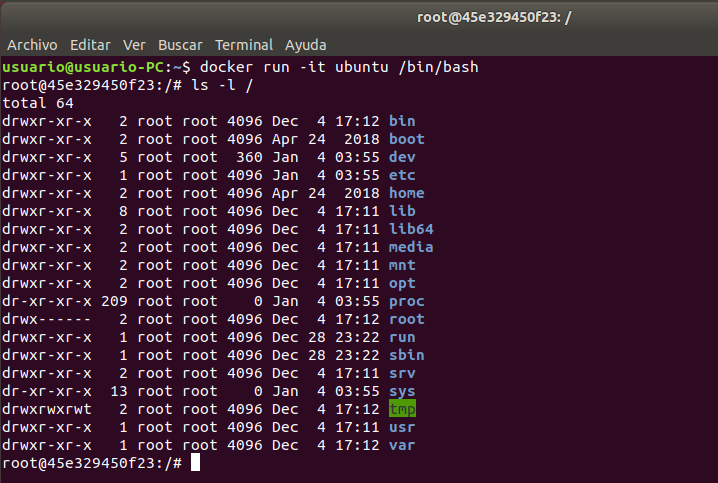
\includegraphics[width=\linewidth]{Trabajo/RecursosEducativos/RE05_Docker/Gestion_basica/REDocker_Gestion9.png}
	\vspace{-0.2cm}
	\caption{Salida comando docker run ubuntu ls -l /}
	\label{fig:DockerGestion9}
\end{figure}

Para poder salir de la terminal del contenedor se puede hacer de dos formas:
\begin{itemize}
    \item exit: El comando exit detiene la ejecución del contenedor y se regresará a la terminal del host.
    \item Ctrl+p+q: Al escribir la combinación de teclas se regresará a la terminal del host sin detener la ejecución del host.
\end{itemize}
%%%%%%%%%%%%%%%%%%%%%%%%%%%%%%%%%
%% INICIAR Y DETENER UN CONTENEDOR 
%%%%%%%%%%%%%%%%%%%%%%%%%%%%%%%%%
\textbf{Detener y reanudar contenedores}
Para detener la ejecución de un contenedor se utiliza el comando stop, pasando como argumento el identificador o el nombre del contenedor, de la siguiente forma

\begin{commandshell} docker stop 45e329450f23 \end{commandshell}

En caso de ser necesario, es posible detener todos los contenedores del host utilizando el comando stop de la siguiente forma

\begin{commandshell} docker stop \$(docker ps -a -q) \end{commandshell}

Para reanudar la ejecución de un contenedor que previamente ha terminado su ejecución se utiliza el comando start, pasando como argumento el identificador o el nombre del contenedor de la siguiente forma 

\begin{commandshell} docker start 45e329450f23 \end{commandshell}

\textbf{Conectarse a un contenedor}
Para conectarse a un contenedor que se encuentra en ejecución se utiliza el comando attach, pasando como argumento el identificador o nombre del contenedor de la siguiente forma

\begin{commandshell} docker attach 45e329450f23 \end{commandshell}

En la figura \ref{fig:DockerGestion10} se puede observar la conexión y ejecución del comando ls en un contenedor que se encontraba previamente en ejecución.

\begin{figure}[!hbtp]
	\centering
	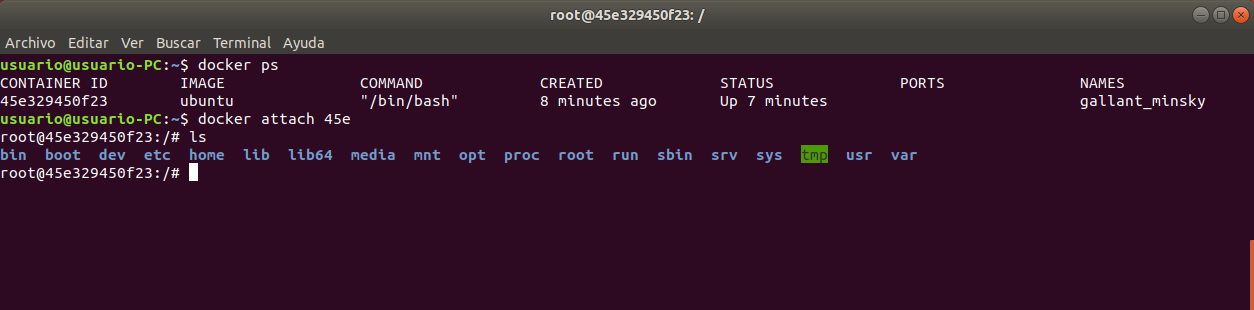
\includegraphics[width=\linewidth]{Trabajo/RecursosEducativos/RE05_Docker/Gestion_basica/REDocker_Gestion10.png}
	\vspace{-0.2cm}
	\caption{Conexión a contenedor en ejecución}
	\label{fig:DockerGestion10}
\end{figure}

%%%%%%%%%%%%%%%%%%%%%%%%%%%%%%%%%%%
%% ELIMINAR IMAGENES Y CONTENEDORES
%%%%%%%%%%%%%%%%%%%%%%%%%%%%%%%%%%%%
\textbf{Eliminar imágenes y contenedores}

Para eliminar un contenedor se requiere que este no se encuentre en ejecución, el comando rm se utiliza para eliminar un contenedor ingresando como argumento el identificador o el nombre del contenedor, de la siguiente forma
\begin{commandshell} docker rm 45e329450f23 \end{commandshell}

En caso de ser necesario, se pueden eliminar todos los contenedores del host utilizando el siguiente comando 
\begin{commandshell} docker rm $(docker ps -a -q)$ \end{commandshell}

Para eliminar una imagen que se encuentra descargada localmente se requiere que esta no tenga contenedores asociados. El comando para realizar la eliminación es rmi y recibe como argumento el identificador de la imagen a eliminar, de la siguiente forma

\begin{commandshell} docker rmi ubuntu \end{commandshell}

En caso de ser necesario, se pueden eliminar todas las imagenes del host utilizando el siguiente comando 
\begin{commandshell}docker rmi \$(docker images -q)\end{commandshell}

%%%%%%%%%%%%%%%%%%%%%%%%%%%%%%%%%%%
%% CONTENEDOR PERSONALIZADO 
%%%%%%%%%%%%%%%%%%%%%%%%%%%%%%%%%%%%
\textbf{Contenedor personalizado}
Para personalizar un contenedor se debe tener una conexión interactiva utilizando el siguiente comando
\begin{commandshell}docker run ubuntu /bin/bash \end{commandshell}

Una vez conectado al contenedor se procede a realizar las modificaciones necesarias, como la instalación de librerías, cambio de variables de entorno, gestión de archivos y directorios, un ejemplo sería la ejecución de los siguientes comandos
\begin{commandshellroot}
apt update
apt install net-tools
apt install nano
\end{commandshellroot}

%%%%%%%%%%%%%%%%%%%%%%%%%%%%%%%%%%%
%% IMAGEN PERSONALIZADA 
%%%%%%%%%%%%%%%%%%%%%%%%%%%%%%%%%%%%
\textbf{Imagen personalizada}
Para la creación de una imagen personalizada se utiliza el comando commit, el cual recibe como argumentos el identificador o nombre del contenedor y el nombre que va tener la imagen personalizada, como se puede ver en el siguiente comando

\begin{commandshell}docker commit 407b4c719d91 ubuntu-personalizado \end{commandshell}

En la figura \ref{fig:DockerGestion11} se puede observar la creación de una imagen personalizada y la verificación de que esta se encuentra disponible para su uso.

\begin{figure}[!hbtp]
	\centering
	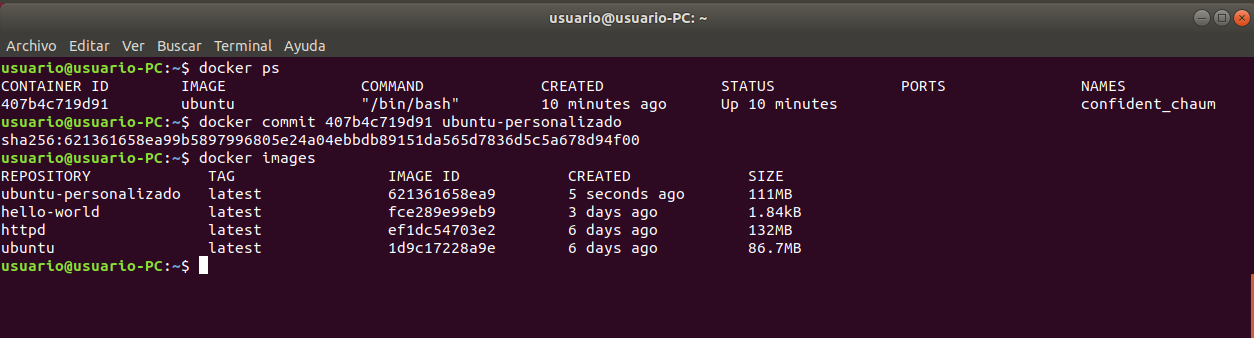
\includegraphics[width=\linewidth]{Trabajo/RecursosEducativos/RE05_Docker/Gestion_basica/REDocker_Gestion11.png}
	\vspace{-0.2cm}
	\caption{Creación imagen personalizada}
	\label{fig:DockerGestion11}
\end{figure}

\subsection{Caso resuelto}
El caso que se va realizar es la personalización de un contenedor y una imagen basada en ubuntu instalando el servidor Apache Web Server.

Para realizar la descarga de la imagen correspondiente se utiliza el comando

\begin{commandshell} docker pull ubuntu \end{commandshell}

Paso siguiente se crea un nuevo contenedor con el nombre de ubuntu-apache iniciando una consola interactiva, de la siguiente forma

\begin{commandshell} docker run --name ubuntu-apache -it ubuntu /bin/bash \end{commandshell}

Al estar en la terminal del contenedor se ejecutan los siguientes comandos para la instalación del servicio web de la siguiente forma 
\begin{commandshellroot}
apt update
apt install apache2
service start apache2
\end{commandshellroot}

Luego de instalados los paquetes necesarios e iniciado el servicio, se debe volver a la terminal del host y crear una imagen a partir del contenedor modificado previamente utilizando el siguiente comando

\begin{commandshell}
docker commit -c='CMD ["apache2ctl" , "-DFOREGROUND"]' \\
    -c 'EXPOSE 80' ubuntu-apache imagen-apache
\end{commandshell}

En el comando mostrado anteriormente, se realizan dos modificaciones importantes a la imagen: 
\begin{itemize}
    \item -c='CMD ["apache2ctl" , "-DFOREGROUND"]': Se agrega que al momento de su inicio se ejecute el servicio de apache en segundo plano.
    \item -c 'EXPOSE 80': Expone el puerto 80 de los contenedores creados con dicha imagen.
\end{itemize}

En la figura \ref{fig:DockerCaso1} se muestran la creación de la imagen personalizada a partir del contenedor ubuntu-apache.

\begin{figure}[!hbtp]
	\centering
	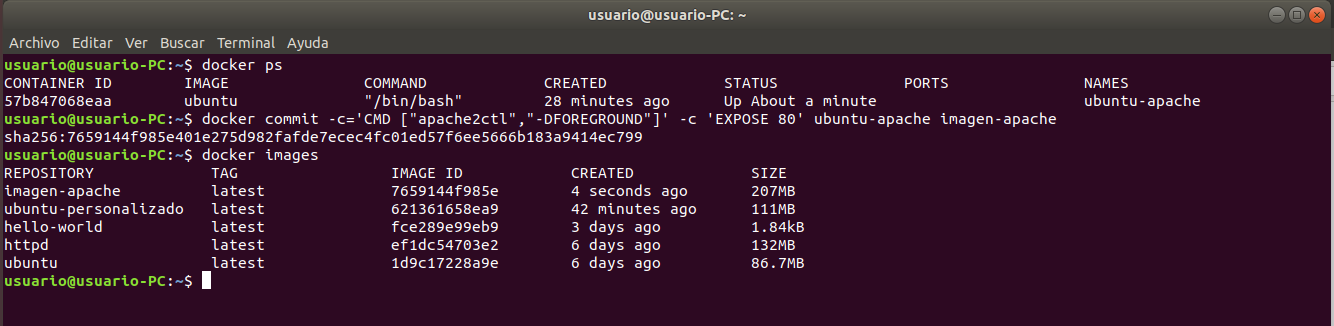
\includegraphics[width=\linewidth]{Trabajo/RecursosEducativos/RE05_Docker/Caso_resuelto/REDocker_Caso1.png}
	\vspace{-0.2cm}
	\caption{Creación imagen personalizada}
	\label{fig:DockerCaso1}
\end{figure}

Teniendo la imagen llamada imagen-apache disponible se procede a crear un nuevo contenedor basado en ella, utilizando el siguiente comando:

\begin{commandshell}
docker run --name nuevo-apache -d -p 8080:80 imagen-apache
\end{commandshell}

En el comando utilizado anteriormente resalta lo siguiente:
\begin{itemize}
    \item -d: Ejecuta el contenedor en segundo plano.
    \item -p 8080:80 : Permite que el puerto 80 del contenedor sea accedido a través del puerto 8080 del host.
    \item --name nuevo-apache: Nombre del contenedor.
\end{itemize}

En la figura \ref{fig:DockerCaso2} se muestra el proceso de creación y verificación del funcionamiento del contenedor llamado nuevo-ubuntu.

\begin{figure}[!hbtp]
	\centering
	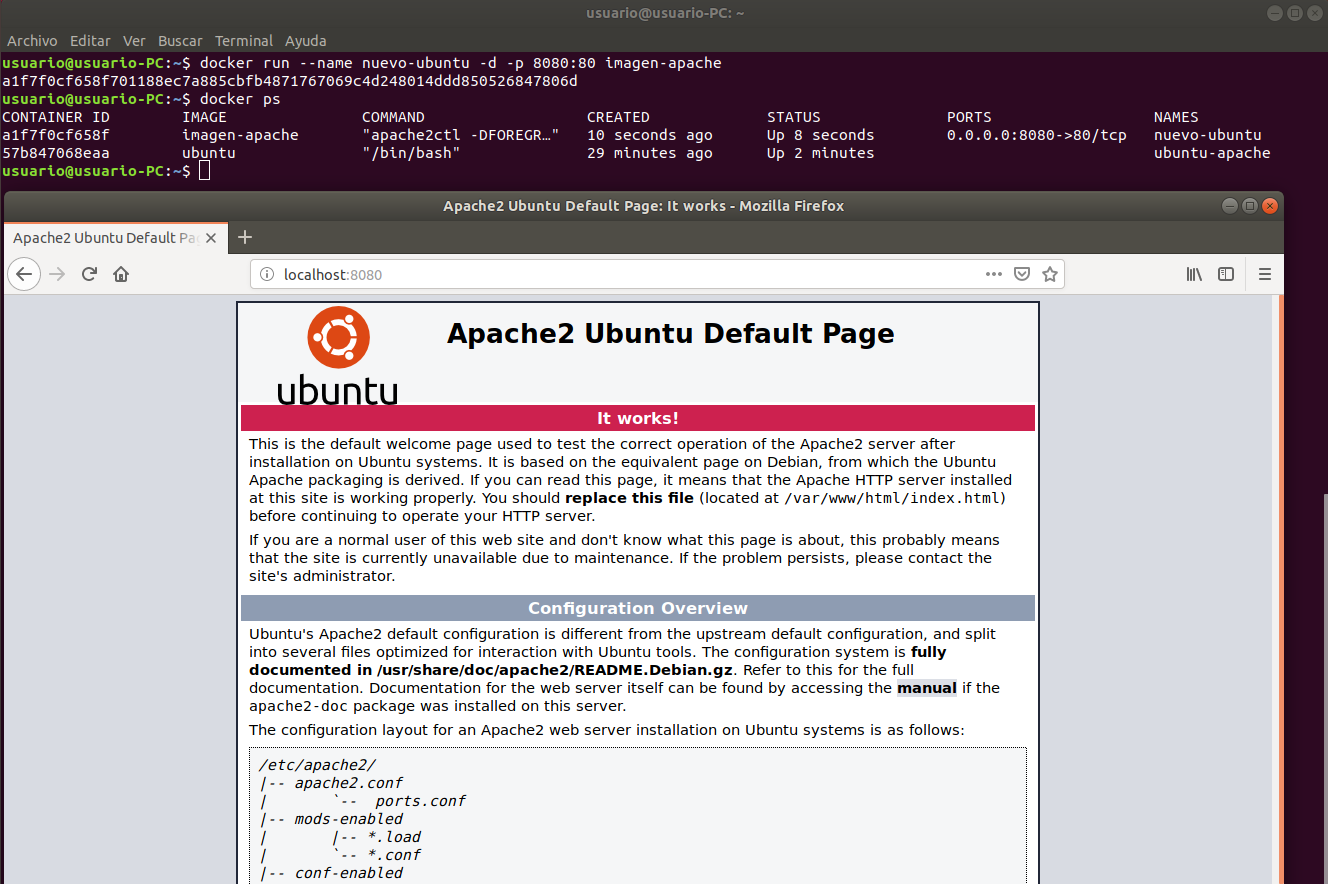
\includegraphics[width=\linewidth]{Trabajo/RecursosEducativos/RE05_Docker/Caso_resuelto/REDocker_Caso2.png}
	\vspace{-0.2cm}
	\caption{Creación imagen personalizada}
	\label{fig:DockerCaso2}
\end{figure}



\subsection{Recurso Educativo 1}

- Objetivo (Competencia)\\

- Arquitectura tecnológica\\

- Aspectos técnicos generales\\

- Proceso de instalación\\

- Gestión básica de la herramienta\\

- Ejercicios (caso) resuelto\\

Ejercicios propuestos\\
- Ejercicio propuesto 1\\
- Ejercicio propuesto 2\\



\subsection{Recurso Educativo 2}
Arquitectura tecnológica
\\\\
Aspectos técnicos generales
\\\\
Proceso de instalación
\\\\
Gestión básica de la herramienta
\\\\
Caso resuelto: 
\\\\

Ejercicios propuestos: 
\\\\

Ejercicio propuesto 1
\\\\

Ejercicio propuesto 2









\section{Para-Virtualización}
\subsection{Recurso Educativo 1}
Arquitectura tecnológica
\\\\
Aspectos técnicos generales
\\\\
Proceso de instalación
\\\\
Gestión básica de la herramienta
\\\\
Caso resuelto: 
\\\\

Ejercicios propuestos: 
\\\\

Ejercicio propuesto 1
\\\\

Ejercicio propuesto 2

....

\subsection{Recurso Educativo 2}
Arquitectura tecnológica
\\\\
Aspectos técnicos generales
\\\\
Proceso de instalación
\\\\
Gestión básica de la herramienta
\\\\
Caso resuelto: 
\\\\

Ejercicios propuestos: 
\\\\

Ejercicio propuesto 1
\\\\

Ejercicio propuesto 2
....
\section{Virtualización basada en Sistema Operativo}
\subsection{Recurso Educativo 1}
Arquitectura tecnológica
\\\\
Aspectos técnicos generales
\\\\
Proceso de instalación
\\\\
Gestión básica de la herramienta
\\\\
Caso resuelto: 
\\\\

Ejercicios propuestos: 
\\\\

Ejercicio propuesto 1
\\\\

Ejercicio propuesto 2

....

\subsection{Recurso Educativo 2}
Arquitectura tecnológica
\\\\
Aspectos técnicos generales
\\\\
Proceso de instalación
\\\\
Gestión básica de la herramienta
\\\\
Caso resuelto: 
\\\\

Ejercicios propuestos: 
\\\\

Ejercicio propuesto 1
\\\\

Ejercicio propuesto 2
....



\chapterimage{chapterImage} % Chapter heading image Anexos
\chapter*{Anexos}
\addcontentsline{toc}{chapter}{\textcolor{ocre}{Anexos}}

\section{Anexo1: Instalación de Oracle Virtual Box}
A continuación se presenta un conjunto de imágenes que muestran la secuencia de pasos realizados en el proceso de instalación de la herramienta \textit{Oracle Virtual Box}\\

\begin{center}
		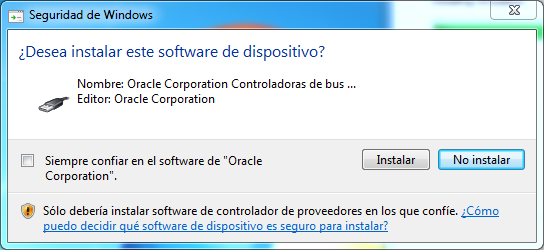
\includegraphics[width=\linewidth]{Trabajo/Anexo01/oracleVirtualBox01.png}
		
		\includegraphics[width=\linewidth]{Trabajo/Anexo01/oracleVirtualBox02.png}

		\includegraphics[width=\linewidth]{Trabajo/Anexo01/oracleVirtualBox03.png}

		\includegraphics[width=\linewidth]{Trabajo/Anexo01/oracleVirtualBox04.png}

		\includegraphics[width=\linewidth]{Trabajo/Anexo01/oracleVirtualBox05.png}

		\includegraphics[width=\linewidth]{Trabajo/Anexo01/oracleVirtualBox06.png}

		\includegraphics[width=\linewidth]{Trabajo/Anexo01/oracleVirtualBox07.png}

		\includegraphics[width=\linewidth]{Trabajo/Anexo01/oracleVirtualBox08.png}
\end{center}


Anexo2: Resultados de la aplicación del Modelo Probit


\begin{center}
	\includegraphics[height=6.5cm]{chapterImage}
\end{center}
%----------------

%----------------------------------------------------------------------------------------
%	BIBLIOGRAPHY
%----------------------------------------------------------------------------------------

%\chapterimage{ima1} % Chapter heading image
%Anexos

\chapter*{Bibliografía}
\addcontentsline{toc}{chapter}{\textcolor{ocre}{Bibliografía}}
%\section*{Books}
%\addcontentsline{toc}{section}{Books}
%\printbibliography[heading=bibempty,type=book]
%\addcontentsline{toc}{section}{Article}
%\printbibliography[heading=bibempty,type=article]
\printbibliography[heading=bibempty]




%----------------------------------------------------------------------------------------
%	INDEX
%----------------------------------------------------------------------------------------

%%\cleardoublepage
%%\phantomsection
%%\setlength{\columnsep}{0.75cm}
%%\addcontentsline{toc}{chapter}{\textcolor{ocre}{Índice Alfabético}}
%%\printindex

%----------------------------------------------------------------------------------------

\end{document}